\documentclass{INTERSPEECH2023}

% **************************************
% *    DOUBLE-BLIND REVIEW SETTINGS    *
% **************************************
% Comment out \interspeechcameraready when submitting the 
% paper for review.
% If your paper is accepted, uncomment this to produce the
%  'camera ready' version to submit for publication.
\interspeechcameraready 

% imports
\usepackage[acronym,toc,shortcuts,nonumberlist]{glossaries}
\usepackage{multirow}
\usepackage{pgfplots}
\usepackage{siunitx}
\usepackage{url}
\usepackage{xcolor}

\setlength{\tabcolsep}{2pt} % Narrower tables. Default value: 6pt

% Acronym definitions.
% --------------------
% To disable certain acronyms without removing them everywhere, see this instructions:
% https://tex.stackexchange.com/q/424462/7396
%A
\newacronym{AM}{AM}{acoustic model}
\newacronym{AMI}{AMI}{Augmented Multi-party Interaction}
\newacronym{ARQ}{ARQ}{automatic repeat request}
\newacronym{ASR}{ASR}{automatic speech recognition}
%B
\newacronym[longplural={bi-directional long-short term memories}]{BLSTM}{BLSTM}{bi-directional long-short term memory}
\newacronym{BSS}{BSS}{blind speech separation}
%C
\newacronym{CART}{CART}{classification and regression tree}
\newacronym{CCA}{CCA}{canonical correlation analysis}
\newacronym{CE}{CE}{cross entropy}
\newacronym{CER}{CER}{character error rate}
\newacronym{CDp}{CDp}{context dependent phoneme}
\newacronym{CNN}{CNN}{convolutional neural network}
\newacronym{CPC}{CPC}{contrastive predictive coding}
\newacronym{CTC}{CTC}{connectionist temporal classification}
%D
\newacronym{DCT}{DCT}{discrete cosine transform}
\newacronym{DL}{DL}{deep learning}
\newacronym{DNN}{DNN}{deep neural network}
\newacronym{DNN-HMM}{DNN-HMM}{deep neural network hidden Markov model}
%E
\newacronym{ELBO}{ELBO}{evidence lower bound}
\newacronym{EM}{EM}{expectation maximization}
%F
\newacronym{FE}{FE}{feature extractor}
\newacronym{FIR}{FIR}{finite impulse response}
\newacronym{FFNN}{FFNN}{feed-forward neural network}
\newacronym{fCE}{fCE}{frame-wise cross-entropy}
%G
\newacronym{G2P}{G2P}{grapheme-to-phoneme conversion}
\newacronym{GAN}{GAN}{generative adversarial network}
\newacronym{GMM}{GMM}{Gaussian mixture model}
\newacronym{GMM-HMM}{GMM-HMM}{Gaussian mixture model hidden Markov model}
\newacronym{GPU}{GPU}{graphics processing unit}
%H
\newacronym{HMM}{HMM}{hidden Markov model}
%I
\newacronym{IHM}{IHM}{individual headset microphones}
\newacronym{IIR}{IIR}{infinite impulse response}
%L
\newacronym{LAS}{LAS}{listen-attend-spell}
\newacronym{LC-BLSTM}{LC-BLSTM}{latency-controlled bidirectional long-short term memory}
\newacronym{LDA}{LDA}{linear discriminant analysis}
\newacronym{LM}{LM}{language model}
\newacronym[longplural={long-short term memories}]{LSTM}{LSTM}{long-short term memory}
%M
\newacronym{MDM}{MDM}{multiple distant microphones}
\newacronym{MFCC}{MFCC}{Mel-frequency cepstral coefficients}
\newacronym{MHSA}{MHSA}{multi-head self-attention}
\newacronym{MRES}{MRES}{multi-resolutional}
\newacronym{MT}{MT}{machine translation}
%N
\newacronym{NLP}{NLP}{natural language processing}
\newacronym{NN}{NN}{neural network}
%O
\newacronym{OOV}{OOV}{out-of-vocabulary}
\newacronym{OCLR}{OCLR}{one-cycle learning rate}
%P
\newacronym{PC2}{$\text{PC}^{\text{2}}$}{Paderborn Center for Parallel Computing}

%R
\newacronym{RNA}{RNA}{recurrent neural aligner}
\newacronym{RNN}{RNN}{recurrent neural network}
\newacronym{RSAN}{RSAN}{recurrent selective attention network}
%S
\newacronym{SAT}{SAT}{speaker adaptive training}
\newacronym{SDM}{SDM}{single distant microphone}
\newacronym{SDR}{SDR}{signal-to-distortion ratio}
\newacronym{SC}{SC}{supervised convolutional}
\newacronym{SCF}{SCF}{supervised convolutional features}
\newacronym{sMBR}{sMBR}{state-level minimum Bayes risk}
\newacronym{STFT}{STFT}{short time Fourier transform}
%T
\newacronym{TDNN}{TDNN}{time delay neural network}
\newacronym[longplural={time-frequencies}]{tf}{tf}{time-frequency}
%U
%V
\newacronym{VAD}{VAD}{voice activity detection}
\newacronym{VGG}{VGG}{TODO needs to be added}
\newacronym{VTLN}{VTLN}{vocal tract length normalization}
%W
\newacronym{cpWER}{cpWER}{concatenated minimum-permutation word error rate}
\newacronym{WER}{WER}{word error rate}
\newacronym{WERR}{WERR}{word error rate reduction}
\newacronym{WP}{WP}{work package}
\newacronym{WPE}{WPE}{weighted prediction error}
\newacronym{WSJ}{WSJ}{Wall Street Journal}

% regular commands
\newcommand\refsec[1]{section~\ref{#1}}
\newcommand\refSec[1]{Section~\ref{#1}}
\newcommand\refcha[1]{chapter~\ref{#1}}
\newcommand\refCha[1]{Chapter~\ref{#1}}
\newcommand\refeqn[1]{equation~\ref{#1}}
\newcommand\refEqn[1]{Equation~\ref{#1}}
\newcommand\reffig[1]{figure~\ref{#1}}
\newcommand\refFig[1]{Figure~\ref{#1}}
\newcommand\refalg[1]{algorithm~\ref{#1}}
\newcommand\refAlg[1]{Algorithm~\ref{#1}}
\newcommand\refapp[1]{appendix~\ref{#1}}
\newcommand\refApp[1]{Appendix~\ref{#1}}
\newcommand\reftab[1]{table~\ref{#1}}
\newcommand\refTab[1]{Table~\ref{#1}}
\newcommand{\citearxiv}[1]{\footnote{\bibentry{#1}}}
\newcommand{\ms}[1]{\SI{#1}{\milli\second}}
\newcommand{\devclean}{\textit{dev-clean}\xspace}
\newcommand{\devother}{\textit{dev-other}\xspace}
\newcommand{\testclean}{\textit{test-clean}\xspace}
\newcommand{\testother}{\textit{test-other}\xspace}
\newcommand{\relu}{ReLU\xspace}
\newcommand{\transformer}{\textit{Transformer}\xspace}
\newcommand{\conformer}{\textit{Conformer}\xspace}
\newcommand{\wv}{\textit{wav2vec}\xspace}
\newcommand{\wvtwo}{\textit{wav2vec 2.0}\xspace}  % cannot use numbers in macro, see https://texfaq.org/FAQ-linmacnames
\newcommand{\lrg}{\textit{Large}\xspace}  % \large is already used
\newcommand{\fe}{\gls{FE}\xspace}
\newcommand{\fes}{\glspl{FE}\xspace}
\newcommand{\glsarticle}[1]{\ifglsused{#1}{an}{a} \gls{#1}}
\newcommand{\Glsarticle}[1]{\ifglsused{#1}{An}{A} \gls{#1}}
\newcommand{\addref}{\textbf{[*]}\xspace}
\newcommand{\comment}[1]{{\textit{\color{blue}#1}}}
\newcommand{\draft}[1]{{\color{gray}#1}}
\newcommand{\question}[1]{{\color{red}#1}}
\newcommand{\TODO}[1]{{\color{red}TODO #1}}


\title{Comparative Analysis of the wav2vec 2.0 Feature Extractor}
\name{Peter Vieting$^{1}$, Ralf Schl\"uter$^{1,2}$, Hermann Ney$^{1,2}$}
\address{
  $^1$RWTH Aachen University, Germany\\
  $^2$AppTek GmbH, Germany}
\email{\{vieting,schlueter,ney\}@cs.rwth-aachen.de}

\begin{document}

\maketitle
 
\begin{abstract}
Raw waveform modeling is an interesting research topic for \gls{ASR}.
\wvtwo has seen large success recently and makes use of a convolutional \fe which operates directly on the speech waveform.
Typically, this \fe is seen as part of the overall architecture, but this work investigates this component specifically.
It is used as a replacement for classical feature extraction methods in a \gls{CTC} setup and compared to an alternative neural \fe approach.
Finally, we analyze the learned representations of both neural \fes.
\end{abstract}
\noindent\textbf{Index Terms}: speech recognition, feature extraction, raw waveform modeling


\section{Introduction}
\glspl{AM} for \gls{ASR} traditionally makes use of hand-designed feature extraction methods like log Mel filterbank features \addref or Gammatone features \cite{schlueter:icassp07}.
These techniques are motivated by insights into the properties of the human auditory system.
However, their fixed design inevitably leads to information loss during the feature extraction.

This issue can be addressed by neural \fes.
Since their parameters are learned during training, these \fes can adapt to the need of \glspl{AM} and the loss of particularly helpful information may be avoided.
A number of works have been proposed in this direction, often using convolutional \glspl{NN} \addref but also applying parametrized functions \cite{ravanelli2018sincnet} and other architectures \cite{sainath2015cldnn}.

Recently, the \wvtwo framework \cite{facebook2020wav2vec2} has received large attention.
It is mainly known for its contrastive self-supervised pre-training, which allows to pre-train a model on large amounts of unlabeled audio data.
Subsequently, it can be fine-tuned for a specific downstream task at hand.
While the context network with multiple \transformer blocks constitutes the major part of the architecture, the \wvtwo model also makes use of a convolutional feature encoder.
\TODO{feature encoder vs. \fe here.}

While the \wvtwo \fe is similar to other neural feature extraction methods, it is not yet closely studied in the literature.
\cite{choi2022w2v2fe} studies the feature encoder by feeding synthesized sine waves.
The authors observe that enough temporal detail is obtained and information about fundamental frequencies is represented in the model's output.
In particular, they claim that the frequencies are distributed linearly over the Hertz scale, unlike perceptually motivated scales like the Mel scale or the Greenwood function for Gammatone features.
\draft{
Other works that analyze \wvtwo models rather focus on the large \transformer part of the network which operates at a higher level of abstraction \cite{livescu2021wav2vec_analysis}\TODO{updated version and add more papers (references in Choi et al. or Livescu et al.}.
}

\draft{
Highlight contributions of this paper.
}

\section{Related work}
\draft{
Works on raw waveform acoustic modeling.
Think about how to properly reference \cite{vieting2021waveform} without disclosing author information.

Different \wv papers \cite{facebook2019wav2vec, facebook2019vqwav2vec, facebook2020wav2vec2, facebook2020xlsr}.
Describe differences between the approaches.
Besides modifications of the self-supervised training criteria -- moving from the future time step prediction in \cite{facebook2019wav2vec} to masked time step prediction -- and incorporating quantization modules, also the architecture has been revised.
Fully convolutional vs. \transformer.
Differences in \fe.

\cite{facebook2019wav2vec} uses 5 layers with kernel sizes (10, 8, 4, 4, 4) and strides which are always exactly half the kernel size.
All have 512 channels, a group normalization layer with a single group and a \relu nonlinearity.
\cite{facebook2020wav2vec2} uses seven layers with kernel sizes (10, 3, 3, 3, 3, 2, 2), strides (5, 2, 2, 2, 2, 2, 2), and a GELU activation function.
The first layer applies group normalization and finally, layer normalization and a linear projection are added.

\cite{asapp2022performance} investigates different settings for the \wvtwo \fe and shows that the required computation can be significantly reduced while maintaining \TODO{similar} performance.
However, this is always done in the whole \wvtwo framework and not \TODO{what is different to us?}
}

\section{Methods}
This work compares different \fes' applicability for \gls{ASR}.
We always normalize the waveform to zero mean and unit variance before it is input to a \fe.
The \fe is followed by the remaining \gls{AM}.
While the separation between \fe and remaining \gls{AM} is not sharp for neural feature extraction, we always refer to the part that replaces the traditional feature extraction as \fe.

\subsection{Feature Extractors}
\subsubsection{Standard Feature Extraction}
As a reference, we use standard, hand-designed \fes -- namely log Mel filterbank features and Gammatone features.
To compute the log Mel filterbank features, first the \gls{STFT} of the waveform is computed with a window size of \ms{25} and a shift of \ms{10}.
We keep the square of the magnitude and perform Mel warping to obtain a 80-dim vector.
Finally, $\log_{10}$ and normalization are applied.

Gammatone features apply a gammatone filterbank to the pre-emphasized speech signal, perform temporal integration over each channel using a low pass filter, i.e., the Hanning window with a size of \ms{25} and a shift of \ms{10}, compress using the $10^{th}$ root and finally compute the \gls{DCT} of the values \cite{schlueter:icassp07}.
Further, the the resulting 50-dim features are normalized.

\subsubsection{\wvtwo Feature Extractor}
The \gls{FE} of the \wvtwo model \cite{facebook2020wav2vec2} mainly consists of 7 convolutional layers.
They are configured with kernel sizes (10, 3, 3, 3, 3, 2, 2), strides (5, 2, 2, 2, 2, 2, 2), and a GELU activation function.
The first layer applies group normalization and finally, layer normalization and a linear projection is added.
The total receptive field of the \wvtwo \fe is \ms{9999} and the shift between consecutive frames is \ms{20}.
Since the other \fes operate at a shift of \ms{10} and the \wvtwo \fe is built in a modular way, we remove the last layer with a stride of 2 in order to achieve features at the same frame rate.
This reduces the total receptive field to \ms{9999}.

\subsubsection{Supervised Convolutional Features}
As an alternative comparable neural feature extraction method, we use \gls{SC} features \cite{tuske2018:waveform, vieting2021waveform}.
Similarly, a convolutional filterbank with learnable parameters is applied to the waveform.
As in the case of Gammatones, a temporal integration is performed over each channel.
However, in this case multiple filters are used for temporal integration allowing for multi-resolutional processing.
Additionally, these filters are learned during training.
By default, we set the size of the first filterbank to 256, its strides to 10 and the number of channels to 150.
The second convolutional filter applies 5 temporal integration filters with a size of 40 and strides of 16 each.
Since the output of all 5 filters is stacked, we have a resulting feature dimension of 750.
The total receptive field of the \gls{SC} features is \ms{9999}.

\subsection{Acoustic Model}
The \gls{AM} mainly consists of \gls{VGG} \addref blocks for downsampling and 12 \conformer blocks.
The \gls{VGG} downsampling uses three 3x3-convolutional layers with 32, 64 and 64 channels, respectively.
In total, a subsampling factor of 4 in the time dimension is achieved by the strided convolutions so that the \conformer operates on frames with a shift of \SI{40}{\milli\second}.
The feature dimension is reduced by a factor of 2 due to max pooling and then multiplied by the number of channels in the last convolution resulting in a total increase by factor 32 in our case.
\draft{
There is a linear layer and dropout here.
The \conformer blocks should be described here.
}
The configuration follows the setup in \cite{zeineldeen2022robustconformer} \TODO{check!}.

\subsection{Connectionist Temporal Classification}
We use a \gls{CTC} model for our experiments.
It follows the setup described for the \gls{CTC} model in \cite{zhou2022efficient}.
\TODO{Cite Wei's paper and add more description of the CTC model.}
All models are trained in a purely supervised fashion unless explicitly stated otherwise.
\TODO{Do we use an LM?}

\section{Experimental Setup}
\subsection{Data}
We conduct experiments on the 960h LibriSpeech corpus \cite{panayotov2015librispeech}, which consists of read English speech.
For the experiments using a pre-trained \wvtwo \fe, the same 960h were used in pre-training.
\draft{The \gls{LM} was trained on the default LibriSpeech \gls{LM} training data which includes the transcriptions of the training set along with the additional
800M-word text-only data.}
The evaluation is done on the standard \devclean, \devother, \testclean and \testother sets.

\subsection{Training Details}
\draft{We follow the setup in \TODO{Wei's paper} \addref.}
The batch size is 640k samples, which corresponds to \SI{40}{\second} of speech waveform and the gradients are accumulated over 3 steps.
The \TODO{NAdam} optimizer uses a \gls{OCLR} schedule with a peak learning rate of \TODO{X} as described in .
Each model is trained on a single \gls{GPU}.
\TODO{What about chunking? More details needed?}

\section{Results}
The results, namely the \glspl{WER} on the LibriSpeech \textit{dev} and \textit{test} sets, for the different \fes are shown in \refTab{table:features_general}.
We can observe that all are within a close range.
The \gls{SC} features slightly outperform the Gammatone baseline, while log Mel features are again marginally better and the \wvtwo \fe yields the best results.
This demonstrates that learnable neural \fes are competitive with hand-designed methods in a purely supervised setup with 960h of training data.
However, a clear advantage of these techniques cannot be deduced from the experimental results.

\begin{table}[htbp]

\centering
\caption{Comparison of different feature extraction methods for a CTC model on LibriSpeech.}
\label{table:features_general}
\begin{tabular}{|c|c|c|c|S|c|S|c|}
\hline
\multicolumn{2}{|c|}{Feature Extractor} & \multicolumn{2}{c|}{\#Params} & \multicolumn{4}{c|}{{WER [\%]}} \\\cline{5-8}
                 \multicolumn{2}{|c|}{} &         \multicolumn{2}{c|}{} &      \multicolumn{2}{c|}{{dev}} & \multicolumn{2}{c|}{{test}} \\\hline
                                   Type &           Name &                         Total &   FE &                         {clean} & other &                     {clean} & other \\\hline\hline
                                  Fixed &      Gammatone &                         73.7M &  32k &                                 &   7.1 &                             &       \\\cline{2-8}
                                        & Mel Filterbank &                               &      &                                 &   6.9 &                             &       \\\hline
                                     NN &             SC &                         85.2M &  40k &                                 &   7.1 &                             &       \\\cline{2-8}
                                        &    wav2vec 2.0 &                         89.5M & 4.1M &                                 &   6.8 &                             &       \\
\hline
\end{tabular}

\end{table}


\subsection{Model Sizes}
It is striking that the \wv2 \fe uses 100x more parameters than the \gls{SC} architecture.
We therefore study the contribution of its components in \refSec{sec:w2v_components} and increase the number of parameters in the \gls{SC} model in \refSec{sec:scf_size}.
Additionally, the size of the first window operating on the waveform is analyzed in \refSec{sec:scf_first_window}.

\subsubsection{Dissecting the wav2vec 2.0 Feature Extractor}
\label{sec:w2v_components}
To understand where \wvtwo uses the parameters and how much they contribute to the \gls{FE}'s performance, we run it with different configurations.
The results for different widths and depths are shown in \refTab{table:features_w2v_size}.
The kernel sizes and strides were chosen as (10, 3, 3, 3, 3, 2), (5, 2, 2, 2, 2, 2) for 6 layers, (10, 6, 3, 3, 3), (5, 4, 2, 2, 2) for 5 layers, (10, 6, 6, 3), (5, 4, 4, 2) for 4 layers, (20, 6, 6), (10, 4, 4) for 3 layers and (32, 20), (16, 10) for 2 layers.
The results show that a larger inner dimension leads to a better performance
In contrast, no major effect can be observed regarding the number of layers.
We also tried a variant with only one layer using kernel size 320 and stride 160 which did not converge.
The final projection, which comprises about \TODO{400k} parameters, additionally improves the performance as shown in \refTab{table:features_w2v_proj}.

\begin{table}[htbp]

\centering
\caption{Studying the effect of the wav2vec 2.0 feature extractor's width and depth.}
\label{table:features_w2v_size}
\begin{tabular}{|c|c|c|c|c|S|c|}
\hline
\#Layers & Dim & \#Params FE & \multicolumn{4}{c|}{{WER [\%]}} \\\cline{4-7}
         &     &             &      \multicolumn{2}{c|}{{dev}} & \multicolumn{2}{c|}{{test}} \\\cline{4-7}
         &     &             &                         {clean} & other &                     {clean} & other \\\hline\hline
       6 & 512 &        4.1M &                                 &   6.8 &                             &       \\\cline{2-7}
         & 256 &        1.1M &                                 &   7.1 &                             &       \\\cline{2-7}
         & 128 &        330k &                                 &   7.2 &                             &       \\\cline{2-7}
         &  64 &        108k &                                 &   7.4 &                             &       \\\hline
       5 & 512 &        4.3M &                                 &   7.1 &                             &       \\\cline{2-7}
         &  64 &        112k &                                 &   7.4 &                             &       \\\hline
       4 & 512 &        4.3M &                                 &   7.0 &                             &       \\\cline{2-7}
         &  64 &        112k &                                 &   7.2 &                             &       \\\hline
       3 & 512 &        3.6M &                                 &   6.9 &                             &       \\\cline{2-7}
         &  64 &        101k &                                 &   7.4 &                             &       \\\hline
       2 & 512 &        5.6M &                                 &   7.1 &                             &       \\\cline{2-7}
         &  64 &        134k &                                 &   7.6 &                             &       \\
\hline
\end{tabular}

\end{table}


\begin{table}[htbp]

\centering
\caption{Studying the effect of the final projection in the wav2vec 2.0 feature extractor.}
\label{table:features_w2v_proj}
\begin{tabular}{|c|c|S|c|S|c|}
\hline
Proj. & \#Params FE & \multicolumn{4}{c|}{{WER [\%]}} \\\cline{3-6}
      &             &      \multicolumn{2}{c|}{{dev}} & \multicolumn{2}{c|}{{test}} \\\cline{3-6}
      &             &                         {clean} & other &                     {clean} & other \\\hline\hline
   No &        3.7M &                             2.9 &   7.0 &                             &       \\\hline
  Yes &        4.1M &                             2.9 &   6.8 &                             &   7.5 \\
\hline
\end{tabular}

\end{table}


\subsubsection{\draft{Inner Dimensions}}
\label{sec:scf_size}
As a larger inner dimension clearly showed better performance for the \wvtwo \gls{FE}, we increase the inner dimensions of the \gls{SC} features as well.
However, as shown in \refTab{table:features_scf_size}, neither increasing the number of filters operating on the waveform nor the number of kernels for the multi-resolutional temporal integration helps to improve the performance.
Note that the number of parameters of the full model is even larger than for the \wvtwo model in \refTab{table:features_general}, however, a large portion of those parameters is consumed by the linear projection of the features after the \gls{VGG} block.

\begin{table}[htbp]

\centering
\caption{Comparison of different inner dimensions for learnable \acrfull{SC} feature extraction.}
\label{table:features_scf_size}
\begin{tabular}{|c|c|c|c|S|}
\hline
 \#Waveform & \#Temp. Integr. & \multicolumn{2}{c|}{\#Params} & {WER} \\\cline{3-4}
Filterbanks &         Kernels &                         Total &  FE &       \\\hline
          5 &             100 &                         81.1M & 27k &   7.1 \\\cline{2-5}
            &             150 &                         85.2M & 40k &   7.1 \\\cline{2-5}
            &             200 &                         89.3M & 53k &   7.1 \\\cline{2-5}
            &             250 &                         93.4M & 67k &   7.3 \\\hline
          6 &             150 &                         87.7M & 40k &   7.3 \\\cline{1-1}\cline{3-5}
          7 &                 &                         90.1M & 41k &   7.1 \\
\hline
\end{tabular}

\end{table}


\subsubsection{First Layer Window Size}
\label{sec:scf_first_window}
Furthermore, the effect of the first layer's window size is studied and the results are shown in \refTab{table:features_window_size}.
They suggest that smaller window sizes than in \cite{tuske2018:waveform} perform better in the context of a \conformer \gls{CTC} model.
In particular, it does not seem to be necessary to cover one full \draft{pitch period (max. fundamental period) \TODO{check detailed explanation} which is around \ms{16}}.
Instead, the best result is achieved with a window size of \ms{10}.
Note that all experiments in \refSec{sec:scf_size} use a window size of \ms{16}.

\begin{table}[htbp]

\centering
\caption{Comparison of different sizes for the layer which operates directly on the waveform in the learnable \acrfull{SC} feature extraction.}
\label{table:features_window_size}
\begin{tabular}{|c|c|S|c|S|c|}
\hline
\multicolumn{2}{|c|}{Window Size} & \multicolumn{4}{c|}{{WER [\%]}} \\\cline{3-6}
           \multicolumn{2}{|c|}{} &      \multicolumn{2}{c|}{{dev}} & \multicolumn{2}{c|}{{test}} \\\hline
                       in samples & in \si{\milli\second} &                         {clean} & other &                     {clean} & other \\\hline\hline
                               64 &                     4 &                             3.0 &   7.2 &                         3.4 &   7.8 \\\hline
                              128 &                     8 &                             3.0 &   7.1 &                         3.3 &   7.6 \\\hline
                              160 &                    10 &                             2.9 &   7.0 &                         3.4 &   7.6 \\\hline
                              256 &                    16 &                             3.0 &   7.1 &                         3.4 &   7.7 \\\hline
                              400 &                    25 &                             2.9 &   7.3 &                         3.4 &   7.7 \\
\hline
\end{tabular}

\end{table}


\subsection{\wvtwo Pre-Training}
The main appeal of the \wvtwo framework is the ability to pre-train the model on unlabeled audio data.
\cite{facebook2020wav2vec2} even reports relative \gls{WER} improvements of about 10\% on the \textit{other} subsets for their experiments on LibriSpeech when pre-training on the same data as used in supervised training compared to pure supervised training from scratch.
Here, we study this effect for the \fe only by using the parameters of an \fe pre-trained on LibriSpeech\footnote{\raggedright\url{https://github.com/facebookresearch/fairseq/blob/main/examples/wav2vec/README.md}}, so no external data is added.
During the supervised training, the \fe weights can be further trained or kept frozen.
As shown in \refTab{table:features_pretraining}, no positive effect can be observed here.
In fact, using a frozen pre-trained \fe shows clearly worse performance than training the \fe purely supervised from scratch.
We hypothesize that the pre-training mainly benefits the \transformer encoder and not the \fe while the mismatch between the \transformer encoder in pre-training and \conformer encoder in our setup could also pose a challenge for the case that the \fe is frozen.

\begin{table}[htbp]

\centering
\caption{Effect of pre-training the wav2vec 2.0 feature extractor using the unsupervised loss on the same data (Librispeech 960h).}
\label{table:features_pretraining}
\begin{tabular}{|c|c|S|}
\hline
\multicolumn{2}{|c|}{Feature Extractor} &       {WER} \\\hline
                              Trainable & Pretrained & {dev-other} \\\hline
                                    yes &         no &         6.8 \\\cline{2-3}
                                        &        yes &         6.9 \\\cline{1-1}\cline{3-3}
                                     no &            &         7.1 \\
\hline
\end{tabular}

\end{table}


\subsection{Frequency Response of Learned Filters}
%% Creator: Matplotlib, PGF backend
%%
%% To include the figure in your LaTeX document, write
%%   \input{<filename>.pgf}
%%
%% Make sure the required packages are loaded in your preamble
%%   \usepackage{pgf}
%%
%% Also ensure that all the required font packages are loaded; for instance,
%% the lmodern package is sometimes necessary when using math font.
%%   \usepackage{lmodern}
%%
%% Figures using additional raster images can only be included by \input if
%% they are in the same directory as the main LaTeX file. For loading figures
%% from other directories you can use the `import` package
%%   \usepackage{import}
%%
%% and then include the figures with
%%   \import{<path to file>}{<filename>.pgf}
%%
%% Matplotlib used the following preamble
%%   
%%   \makeatletter\@ifpackageloaded{underscore}{}{\usepackage[strings]{underscore}}\makeatother
%%
\begingroup%
\makeatletter%
\begin{pgfpicture}%
\pgfpathrectangle{\pgfpointorigin}{\pgfqpoint{6.299213in}{3.937008in}}%
\pgfusepath{use as bounding box, clip}%
\begin{pgfscope}%
\pgfsetbuttcap%
\pgfsetmiterjoin%
\definecolor{currentfill}{rgb}{1.000000,1.000000,1.000000}%
\pgfsetfillcolor{currentfill}%
\pgfsetlinewidth{0.000000pt}%
\definecolor{currentstroke}{rgb}{1.000000,1.000000,1.000000}%
\pgfsetstrokecolor{currentstroke}%
\pgfsetdash{}{0pt}%
\pgfpathmoveto{\pgfqpoint{0.000000in}{0.000000in}}%
\pgfpathlineto{\pgfqpoint{6.299213in}{0.000000in}}%
\pgfpathlineto{\pgfqpoint{6.299213in}{3.937008in}}%
\pgfpathlineto{\pgfqpoint{0.000000in}{3.937008in}}%
\pgfpathlineto{\pgfqpoint{0.000000in}{0.000000in}}%
\pgfpathclose%
\pgfusepath{fill}%
\end{pgfscope}%
\begin{pgfscope}%
\pgfsetbuttcap%
\pgfsetmiterjoin%
\definecolor{currentfill}{rgb}{1.000000,1.000000,1.000000}%
\pgfsetfillcolor{currentfill}%
\pgfsetlinewidth{0.000000pt}%
\definecolor{currentstroke}{rgb}{0.000000,0.000000,0.000000}%
\pgfsetstrokecolor{currentstroke}%
\pgfsetstrokeopacity{0.000000}%
\pgfsetdash{}{0pt}%
\pgfpathmoveto{\pgfqpoint{0.375000in}{2.909651in}}%
\pgfpathlineto{\pgfqpoint{3.153078in}{2.909651in}}%
\pgfpathlineto{\pgfqpoint{3.153078in}{3.714786in}}%
\pgfpathlineto{\pgfqpoint{0.375000in}{3.714786in}}%
\pgfpathlineto{\pgfqpoint{0.375000in}{2.909651in}}%
\pgfpathclose%
\pgfusepath{fill}%
\end{pgfscope}%
\begin{pgfscope}%
\pgfpathrectangle{\pgfqpoint{0.375000in}{2.909651in}}{\pgfqpoint{2.778078in}{0.805134in}}%
\pgfusepath{clip}%
\pgfsys@transformshift{0.375000in}{2.909651in}%
\pgftext[left,bottom]{
\includegraphics[interpolate=true,width=2.780000in,height=0.810000in]{figures/first_layer-img0.png}}%
\end{pgfscope}%
\begin{pgfscope}%
\pgfsetbuttcap%
\pgfsetroundjoin%
\definecolor{currentfill}{rgb}{0.000000,0.000000,0.000000}%
\pgfsetfillcolor{currentfill}%
\pgfsetlinewidth{0.803000pt}%
\definecolor{currentstroke}{rgb}{0.000000,0.000000,0.000000}%
\pgfsetstrokecolor{currentstroke}%
\pgfsetdash{}{0pt}%
\pgfsys@defobject{currentmarker}{\pgfqpoint{0.000000in}{-0.048611in}}{\pgfqpoint{0.000000in}{0.000000in}}{%
\pgfpathmoveto{\pgfqpoint{0.000000in}{0.000000in}}%
\pgfpathlineto{\pgfqpoint{0.000000in}{-0.048611in}}%
\pgfusepath{stroke,fill}%
}%
\begin{pgfscope}%
\pgfsys@transformshift{0.885259in}{2.909651in}%
\pgfsys@useobject{currentmarker}{}%
\end{pgfscope}%
\end{pgfscope}%
\begin{pgfscope}%
\definecolor{textcolor}{rgb}{0.000000,0.000000,0.000000}%
\pgfsetstrokecolor{textcolor}%
\pgfsetfillcolor{textcolor}%
\pgftext[x=0.885259in,y=2.812429in,,top]{\color{textcolor}\rmfamily\fontsize{10.000000}{12.000000}\selectfont \(\displaystyle {10}\)}%
\end{pgfscope}%
\begin{pgfscope}%
\pgfsetbuttcap%
\pgfsetroundjoin%
\definecolor{currentfill}{rgb}{0.000000,0.000000,0.000000}%
\pgfsetfillcolor{currentfill}%
\pgfsetlinewidth{0.803000pt}%
\definecolor{currentstroke}{rgb}{0.000000,0.000000,0.000000}%
\pgfsetstrokecolor{currentstroke}%
\pgfsetdash{}{0pt}%
\pgfsys@defobject{currentmarker}{\pgfqpoint{0.000000in}{-0.048611in}}{\pgfqpoint{0.000000in}{0.000000in}}{%
\pgfpathmoveto{\pgfqpoint{0.000000in}{0.000000in}}%
\pgfpathlineto{\pgfqpoint{0.000000in}{-0.048611in}}%
\pgfusepath{stroke,fill}%
}%
\begin{pgfscope}%
\pgfsys@transformshift{1.452214in}{2.909651in}%
\pgfsys@useobject{currentmarker}{}%
\end{pgfscope}%
\end{pgfscope}%
\begin{pgfscope}%
\definecolor{textcolor}{rgb}{0.000000,0.000000,0.000000}%
\pgfsetstrokecolor{textcolor}%
\pgfsetfillcolor{textcolor}%
\pgftext[x=1.452214in,y=2.812429in,,top]{\color{textcolor}\rmfamily\fontsize{10.000000}{12.000000}\selectfont \(\displaystyle {20}\)}%
\end{pgfscope}%
\begin{pgfscope}%
\pgfsetbuttcap%
\pgfsetroundjoin%
\definecolor{currentfill}{rgb}{0.000000,0.000000,0.000000}%
\pgfsetfillcolor{currentfill}%
\pgfsetlinewidth{0.803000pt}%
\definecolor{currentstroke}{rgb}{0.000000,0.000000,0.000000}%
\pgfsetstrokecolor{currentstroke}%
\pgfsetdash{}{0pt}%
\pgfsys@defobject{currentmarker}{\pgfqpoint{0.000000in}{-0.048611in}}{\pgfqpoint{0.000000in}{0.000000in}}{%
\pgfpathmoveto{\pgfqpoint{0.000000in}{0.000000in}}%
\pgfpathlineto{\pgfqpoint{0.000000in}{-0.048611in}}%
\pgfusepath{stroke,fill}%
}%
\begin{pgfscope}%
\pgfsys@transformshift{2.019169in}{2.909651in}%
\pgfsys@useobject{currentmarker}{}%
\end{pgfscope}%
\end{pgfscope}%
\begin{pgfscope}%
\definecolor{textcolor}{rgb}{0.000000,0.000000,0.000000}%
\pgfsetstrokecolor{textcolor}%
\pgfsetfillcolor{textcolor}%
\pgftext[x=2.019169in,y=2.812429in,,top]{\color{textcolor}\rmfamily\fontsize{10.000000}{12.000000}\selectfont \(\displaystyle {30}\)}%
\end{pgfscope}%
\begin{pgfscope}%
\pgfsetbuttcap%
\pgfsetroundjoin%
\definecolor{currentfill}{rgb}{0.000000,0.000000,0.000000}%
\pgfsetfillcolor{currentfill}%
\pgfsetlinewidth{0.803000pt}%
\definecolor{currentstroke}{rgb}{0.000000,0.000000,0.000000}%
\pgfsetstrokecolor{currentstroke}%
\pgfsetdash{}{0pt}%
\pgfsys@defobject{currentmarker}{\pgfqpoint{0.000000in}{-0.048611in}}{\pgfqpoint{0.000000in}{0.000000in}}{%
\pgfpathmoveto{\pgfqpoint{0.000000in}{0.000000in}}%
\pgfpathlineto{\pgfqpoint{0.000000in}{-0.048611in}}%
\pgfusepath{stroke,fill}%
}%
\begin{pgfscope}%
\pgfsys@transformshift{2.586124in}{2.909651in}%
\pgfsys@useobject{currentmarker}{}%
\end{pgfscope}%
\end{pgfscope}%
\begin{pgfscope}%
\definecolor{textcolor}{rgb}{0.000000,0.000000,0.000000}%
\pgfsetstrokecolor{textcolor}%
\pgfsetfillcolor{textcolor}%
\pgftext[x=2.586124in,y=2.812429in,,top]{\color{textcolor}\rmfamily\fontsize{10.000000}{12.000000}\selectfont \(\displaystyle {40}\)}%
\end{pgfscope}%
\begin{pgfscope}%
\pgfsetbuttcap%
\pgfsetroundjoin%
\definecolor{currentfill}{rgb}{0.000000,0.000000,0.000000}%
\pgfsetfillcolor{currentfill}%
\pgfsetlinewidth{0.803000pt}%
\definecolor{currentstroke}{rgb}{0.000000,0.000000,0.000000}%
\pgfsetstrokecolor{currentstroke}%
\pgfsetdash{}{0pt}%
\pgfsys@defobject{currentmarker}{\pgfqpoint{0.000000in}{-0.048611in}}{\pgfqpoint{0.000000in}{0.000000in}}{%
\pgfpathmoveto{\pgfqpoint{0.000000in}{0.000000in}}%
\pgfpathlineto{\pgfqpoint{0.000000in}{-0.048611in}}%
\pgfusepath{stroke,fill}%
}%
\begin{pgfscope}%
\pgfsys@transformshift{3.153078in}{2.909651in}%
\pgfsys@useobject{currentmarker}{}%
\end{pgfscope}%
\end{pgfscope}%
\begin{pgfscope}%
\definecolor{textcolor}{rgb}{0.000000,0.000000,0.000000}%
\pgfsetstrokecolor{textcolor}%
\pgfsetfillcolor{textcolor}%
\pgftext[x=3.153078in,y=2.812429in,,top]{\color{textcolor}\rmfamily\fontsize{10.000000}{12.000000}\selectfont \(\displaystyle {50}\)}%
\end{pgfscope}%
\begin{pgfscope}%
\pgfsetbuttcap%
\pgfsetroundjoin%
\definecolor{currentfill}{rgb}{0.000000,0.000000,0.000000}%
\pgfsetfillcolor{currentfill}%
\pgfsetlinewidth{0.803000pt}%
\definecolor{currentstroke}{rgb}{0.000000,0.000000,0.000000}%
\pgfsetstrokecolor{currentstroke}%
\pgfsetdash{}{0pt}%
\pgfsys@defobject{currentmarker}{\pgfqpoint{-0.048611in}{0.000000in}}{\pgfqpoint{-0.000000in}{0.000000in}}{%
\pgfpathmoveto{\pgfqpoint{-0.000000in}{0.000000in}}%
\pgfpathlineto{\pgfqpoint{-0.048611in}{0.000000in}}%
\pgfusepath{stroke,fill}%
}%
\begin{pgfscope}%
\pgfsys@transformshift{0.375000in}{2.909651in}%
\pgfsys@useobject{currentmarker}{}%
\end{pgfscope}%
\end{pgfscope}%
\begin{pgfscope}%
\definecolor{textcolor}{rgb}{0.000000,0.000000,0.000000}%
\pgfsetstrokecolor{textcolor}%
\pgfsetfillcolor{textcolor}%
\pgftext[x=0.208333in, y=2.861426in, left, base]{\color{textcolor}\rmfamily\fontsize{10.000000}{12.000000}\selectfont \(\displaystyle {0}\)}%
\end{pgfscope}%
\begin{pgfscope}%
\pgfsetbuttcap%
\pgfsetroundjoin%
\definecolor{currentfill}{rgb}{0.000000,0.000000,0.000000}%
\pgfsetfillcolor{currentfill}%
\pgfsetlinewidth{0.803000pt}%
\definecolor{currentstroke}{rgb}{0.000000,0.000000,0.000000}%
\pgfsetstrokecolor{currentstroke}%
\pgfsetdash{}{0pt}%
\pgfsys@defobject{currentmarker}{\pgfqpoint{-0.048611in}{0.000000in}}{\pgfqpoint{-0.000000in}{0.000000in}}{%
\pgfpathmoveto{\pgfqpoint{-0.000000in}{0.000000in}}%
\pgfpathlineto{\pgfqpoint{-0.048611in}{0.000000in}}%
\pgfusepath{stroke,fill}%
}%
\begin{pgfscope}%
\pgfsys@transformshift{0.375000in}{3.312218in}%
\pgfsys@useobject{currentmarker}{}%
\end{pgfscope}%
\end{pgfscope}%
\begin{pgfscope}%
\definecolor{textcolor}{rgb}{0.000000,0.000000,0.000000}%
\pgfsetstrokecolor{textcolor}%
\pgfsetfillcolor{textcolor}%
\pgftext[x=0.208333in, y=3.263993in, left, base]{\color{textcolor}\rmfamily\fontsize{10.000000}{12.000000}\selectfont \(\displaystyle {4}\)}%
\end{pgfscope}%
\begin{pgfscope}%
\pgfsetbuttcap%
\pgfsetroundjoin%
\definecolor{currentfill}{rgb}{0.000000,0.000000,0.000000}%
\pgfsetfillcolor{currentfill}%
\pgfsetlinewidth{0.803000pt}%
\definecolor{currentstroke}{rgb}{0.000000,0.000000,0.000000}%
\pgfsetstrokecolor{currentstroke}%
\pgfsetdash{}{0pt}%
\pgfsys@defobject{currentmarker}{\pgfqpoint{-0.048611in}{0.000000in}}{\pgfqpoint{-0.000000in}{0.000000in}}{%
\pgfpathmoveto{\pgfqpoint{-0.000000in}{0.000000in}}%
\pgfpathlineto{\pgfqpoint{-0.048611in}{0.000000in}}%
\pgfusepath{stroke,fill}%
}%
\begin{pgfscope}%
\pgfsys@transformshift{0.375000in}{3.714786in}%
\pgfsys@useobject{currentmarker}{}%
\end{pgfscope}%
\end{pgfscope}%
\begin{pgfscope}%
\definecolor{textcolor}{rgb}{0.000000,0.000000,0.000000}%
\pgfsetstrokecolor{textcolor}%
\pgfsetfillcolor{textcolor}%
\pgftext[x=0.208333in, y=3.666560in, left, base]{\color{textcolor}\rmfamily\fontsize{10.000000}{12.000000}\selectfont \(\displaystyle {8}\)}%
\end{pgfscope}%
\begin{pgfscope}%
\definecolor{textcolor}{rgb}{0.000000,0.000000,0.000000}%
\pgfsetstrokecolor{textcolor}%
\pgfsetfillcolor{textcolor}%
\pgftext[x=0.152778in,y=3.312218in,,bottom,rotate=90.000000]{\color{textcolor}\rmfamily\fontsize{10.000000}{12.000000}\selectfont Frequency [\si{\kilo\hertz}]}%
\end{pgfscope}%
\begin{pgfscope}%
\pgfsetrectcap%
\pgfsetmiterjoin%
\pgfsetlinewidth{0.803000pt}%
\definecolor{currentstroke}{rgb}{0.000000,0.000000,0.000000}%
\pgfsetstrokecolor{currentstroke}%
\pgfsetdash{}{0pt}%
\pgfpathmoveto{\pgfqpoint{0.375000in}{2.909651in}}%
\pgfpathlineto{\pgfqpoint{0.375000in}{3.714786in}}%
\pgfusepath{stroke}%
\end{pgfscope}%
\begin{pgfscope}%
\pgfsetrectcap%
\pgfsetmiterjoin%
\pgfsetlinewidth{0.803000pt}%
\definecolor{currentstroke}{rgb}{0.000000,0.000000,0.000000}%
\pgfsetstrokecolor{currentstroke}%
\pgfsetdash{}{0pt}%
\pgfpathmoveto{\pgfqpoint{3.153078in}{2.909651in}}%
\pgfpathlineto{\pgfqpoint{3.153078in}{3.714786in}}%
\pgfusepath{stroke}%
\end{pgfscope}%
\begin{pgfscope}%
\pgfsetrectcap%
\pgfsetmiterjoin%
\pgfsetlinewidth{0.803000pt}%
\definecolor{currentstroke}{rgb}{0.000000,0.000000,0.000000}%
\pgfsetstrokecolor{currentstroke}%
\pgfsetdash{}{0pt}%
\pgfpathmoveto{\pgfqpoint{0.375000in}{2.909651in}}%
\pgfpathlineto{\pgfqpoint{3.153078in}{2.909651in}}%
\pgfusepath{stroke}%
\end{pgfscope}%
\begin{pgfscope}%
\pgfsetrectcap%
\pgfsetmiterjoin%
\pgfsetlinewidth{0.803000pt}%
\definecolor{currentstroke}{rgb}{0.000000,0.000000,0.000000}%
\pgfsetstrokecolor{currentstroke}%
\pgfsetdash{}{0pt}%
\pgfpathmoveto{\pgfqpoint{0.375000in}{3.714786in}}%
\pgfpathlineto{\pgfqpoint{3.153078in}{3.714786in}}%
\pgfusepath{stroke}%
\end{pgfscope}%
\begin{pgfscope}%
\definecolor{textcolor}{rgb}{0.000000,0.000000,0.000000}%
\pgfsetstrokecolor{textcolor}%
\pgfsetfillcolor{textcolor}%
\pgftext[x=1.764039in,y=3.798119in,,base]{\color{textcolor}\rmfamily\fontsize{12.000000}{14.400000}\selectfont (a) Gammatone}%
\end{pgfscope}%
\begin{pgfscope}%
\pgfsetbuttcap%
\pgfsetmiterjoin%
\definecolor{currentfill}{rgb}{1.000000,1.000000,1.000000}%
\pgfsetfillcolor{currentfill}%
\pgfsetlinewidth{0.000000pt}%
\definecolor{currentstroke}{rgb}{0.000000,0.000000,0.000000}%
\pgfsetstrokecolor{currentstroke}%
\pgfsetstrokeopacity{0.000000}%
\pgfsetdash{}{0pt}%
\pgfpathmoveto{\pgfqpoint{3.403079in}{2.909651in}}%
\pgfpathlineto{\pgfqpoint{6.181157in}{2.909651in}}%
\pgfpathlineto{\pgfqpoint{6.181157in}{3.714786in}}%
\pgfpathlineto{\pgfqpoint{3.403079in}{3.714786in}}%
\pgfpathlineto{\pgfqpoint{3.403079in}{2.909651in}}%
\pgfpathclose%
\pgfusepath{fill}%
\end{pgfscope}%
\begin{pgfscope}%
\pgfpathrectangle{\pgfqpoint{3.403079in}{2.909651in}}{\pgfqpoint{2.778078in}{0.805134in}}%
\pgfusepath{clip}%
\pgfsys@transformshift{3.403079in}{2.909651in}%
\pgftext[left,bottom]{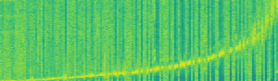
\includegraphics[interpolate=true,width=2.780000in,height=0.810000in]{figures/first_layer-img1.png}}%
\end{pgfscope}%
\begin{pgfscope}%
\pgfsetbuttcap%
\pgfsetroundjoin%
\definecolor{currentfill}{rgb}{0.000000,0.000000,0.000000}%
\pgfsetfillcolor{currentfill}%
\pgfsetlinewidth{0.803000pt}%
\definecolor{currentstroke}{rgb}{0.000000,0.000000,0.000000}%
\pgfsetstrokecolor{currentstroke}%
\pgfsetdash{}{0pt}%
\pgfsys@defobject{currentmarker}{\pgfqpoint{0.000000in}{-0.048611in}}{\pgfqpoint{0.000000in}{0.000000in}}{%
\pgfpathmoveto{\pgfqpoint{0.000000in}{0.000000in}}%
\pgfpathlineto{\pgfqpoint{0.000000in}{-0.048611in}}%
\pgfusepath{stroke,fill}%
}%
\begin{pgfscope}%
\pgfsys@transformshift{3.850554in}{2.909651in}%
\pgfsys@useobject{currentmarker}{}%
\end{pgfscope}%
\end{pgfscope}%
\begin{pgfscope}%
\definecolor{textcolor}{rgb}{0.000000,0.000000,0.000000}%
\pgfsetstrokecolor{textcolor}%
\pgfsetfillcolor{textcolor}%
\pgftext[x=3.850554in,y=2.812429in,,top]{\color{textcolor}\rmfamily\fontsize{10.000000}{12.000000}\selectfont \(\displaystyle {25}\)}%
\end{pgfscope}%
\begin{pgfscope}%
\pgfsetbuttcap%
\pgfsetroundjoin%
\definecolor{currentfill}{rgb}{0.000000,0.000000,0.000000}%
\pgfsetfillcolor{currentfill}%
\pgfsetlinewidth{0.803000pt}%
\definecolor{currentstroke}{rgb}{0.000000,0.000000,0.000000}%
\pgfsetstrokecolor{currentstroke}%
\pgfsetdash{}{0pt}%
\pgfsys@defobject{currentmarker}{\pgfqpoint{0.000000in}{-0.048611in}}{\pgfqpoint{0.000000in}{0.000000in}}{%
\pgfpathmoveto{\pgfqpoint{0.000000in}{0.000000in}}%
\pgfpathlineto{\pgfqpoint{0.000000in}{-0.048611in}}%
\pgfusepath{stroke,fill}%
}%
\begin{pgfscope}%
\pgfsys@transformshift{4.316675in}{2.909651in}%
\pgfsys@useobject{currentmarker}{}%
\end{pgfscope}%
\end{pgfscope}%
\begin{pgfscope}%
\definecolor{textcolor}{rgb}{0.000000,0.000000,0.000000}%
\pgfsetstrokecolor{textcolor}%
\pgfsetfillcolor{textcolor}%
\pgftext[x=4.316675in,y=2.812429in,,top]{\color{textcolor}\rmfamily\fontsize{10.000000}{12.000000}\selectfont \(\displaystyle {50}\)}%
\end{pgfscope}%
\begin{pgfscope}%
\pgfsetbuttcap%
\pgfsetroundjoin%
\definecolor{currentfill}{rgb}{0.000000,0.000000,0.000000}%
\pgfsetfillcolor{currentfill}%
\pgfsetlinewidth{0.803000pt}%
\definecolor{currentstroke}{rgb}{0.000000,0.000000,0.000000}%
\pgfsetstrokecolor{currentstroke}%
\pgfsetdash{}{0pt}%
\pgfsys@defobject{currentmarker}{\pgfqpoint{0.000000in}{-0.048611in}}{\pgfqpoint{0.000000in}{0.000000in}}{%
\pgfpathmoveto{\pgfqpoint{0.000000in}{0.000000in}}%
\pgfpathlineto{\pgfqpoint{0.000000in}{-0.048611in}}%
\pgfusepath{stroke,fill}%
}%
\begin{pgfscope}%
\pgfsys@transformshift{4.782795in}{2.909651in}%
\pgfsys@useobject{currentmarker}{}%
\end{pgfscope}%
\end{pgfscope}%
\begin{pgfscope}%
\definecolor{textcolor}{rgb}{0.000000,0.000000,0.000000}%
\pgfsetstrokecolor{textcolor}%
\pgfsetfillcolor{textcolor}%
\pgftext[x=4.782795in,y=2.812429in,,top]{\color{textcolor}\rmfamily\fontsize{10.000000}{12.000000}\selectfont \(\displaystyle {75}\)}%
\end{pgfscope}%
\begin{pgfscope}%
\pgfsetbuttcap%
\pgfsetroundjoin%
\definecolor{currentfill}{rgb}{0.000000,0.000000,0.000000}%
\pgfsetfillcolor{currentfill}%
\pgfsetlinewidth{0.803000pt}%
\definecolor{currentstroke}{rgb}{0.000000,0.000000,0.000000}%
\pgfsetstrokecolor{currentstroke}%
\pgfsetdash{}{0pt}%
\pgfsys@defobject{currentmarker}{\pgfqpoint{0.000000in}{-0.048611in}}{\pgfqpoint{0.000000in}{0.000000in}}{%
\pgfpathmoveto{\pgfqpoint{0.000000in}{0.000000in}}%
\pgfpathlineto{\pgfqpoint{0.000000in}{-0.048611in}}%
\pgfusepath{stroke,fill}%
}%
\begin{pgfscope}%
\pgfsys@transformshift{5.248916in}{2.909651in}%
\pgfsys@useobject{currentmarker}{}%
\end{pgfscope}%
\end{pgfscope}%
\begin{pgfscope}%
\definecolor{textcolor}{rgb}{0.000000,0.000000,0.000000}%
\pgfsetstrokecolor{textcolor}%
\pgfsetfillcolor{textcolor}%
\pgftext[x=5.248916in,y=2.812429in,,top]{\color{textcolor}\rmfamily\fontsize{10.000000}{12.000000}\selectfont \(\displaystyle {100}\)}%
\end{pgfscope}%
\begin{pgfscope}%
\pgfsetbuttcap%
\pgfsetroundjoin%
\definecolor{currentfill}{rgb}{0.000000,0.000000,0.000000}%
\pgfsetfillcolor{currentfill}%
\pgfsetlinewidth{0.803000pt}%
\definecolor{currentstroke}{rgb}{0.000000,0.000000,0.000000}%
\pgfsetstrokecolor{currentstroke}%
\pgfsetdash{}{0pt}%
\pgfsys@defobject{currentmarker}{\pgfqpoint{0.000000in}{-0.048611in}}{\pgfqpoint{0.000000in}{0.000000in}}{%
\pgfpathmoveto{\pgfqpoint{0.000000in}{0.000000in}}%
\pgfpathlineto{\pgfqpoint{0.000000in}{-0.048611in}}%
\pgfusepath{stroke,fill}%
}%
\begin{pgfscope}%
\pgfsys@transformshift{5.715036in}{2.909651in}%
\pgfsys@useobject{currentmarker}{}%
\end{pgfscope}%
\end{pgfscope}%
\begin{pgfscope}%
\definecolor{textcolor}{rgb}{0.000000,0.000000,0.000000}%
\pgfsetstrokecolor{textcolor}%
\pgfsetfillcolor{textcolor}%
\pgftext[x=5.715036in,y=2.812429in,,top]{\color{textcolor}\rmfamily\fontsize{10.000000}{12.000000}\selectfont \(\displaystyle {125}\)}%
\end{pgfscope}%
\begin{pgfscope}%
\pgfsetbuttcap%
\pgfsetroundjoin%
\definecolor{currentfill}{rgb}{0.000000,0.000000,0.000000}%
\pgfsetfillcolor{currentfill}%
\pgfsetlinewidth{0.803000pt}%
\definecolor{currentstroke}{rgb}{0.000000,0.000000,0.000000}%
\pgfsetstrokecolor{currentstroke}%
\pgfsetdash{}{0pt}%
\pgfsys@defobject{currentmarker}{\pgfqpoint{0.000000in}{-0.048611in}}{\pgfqpoint{0.000000in}{0.000000in}}{%
\pgfpathmoveto{\pgfqpoint{0.000000in}{0.000000in}}%
\pgfpathlineto{\pgfqpoint{0.000000in}{-0.048611in}}%
\pgfusepath{stroke,fill}%
}%
\begin{pgfscope}%
\pgfsys@transformshift{6.181157in}{2.909651in}%
\pgfsys@useobject{currentmarker}{}%
\end{pgfscope}%
\end{pgfscope}%
\begin{pgfscope}%
\definecolor{textcolor}{rgb}{0.000000,0.000000,0.000000}%
\pgfsetstrokecolor{textcolor}%
\pgfsetfillcolor{textcolor}%
\pgftext[x=6.181157in,y=2.812429in,,top]{\color{textcolor}\rmfamily\fontsize{10.000000}{12.000000}\selectfont \(\displaystyle {150}\)}%
\end{pgfscope}%
\begin{pgfscope}%
\pgfsetbuttcap%
\pgfsetroundjoin%
\definecolor{currentfill}{rgb}{0.000000,0.000000,0.000000}%
\pgfsetfillcolor{currentfill}%
\pgfsetlinewidth{0.803000pt}%
\definecolor{currentstroke}{rgb}{0.000000,0.000000,0.000000}%
\pgfsetstrokecolor{currentstroke}%
\pgfsetdash{}{0pt}%
\pgfsys@defobject{currentmarker}{\pgfqpoint{-0.048611in}{0.000000in}}{\pgfqpoint{-0.000000in}{0.000000in}}{%
\pgfpathmoveto{\pgfqpoint{-0.000000in}{0.000000in}}%
\pgfpathlineto{\pgfqpoint{-0.048611in}{0.000000in}}%
\pgfusepath{stroke,fill}%
}%
\begin{pgfscope}%
\pgfsys@transformshift{3.403079in}{2.909651in}%
\pgfsys@useobject{currentmarker}{}%
\end{pgfscope}%
\end{pgfscope}%
\begin{pgfscope}%
\definecolor{textcolor}{rgb}{0.000000,0.000000,0.000000}%
\pgfsetstrokecolor{textcolor}%
\pgfsetfillcolor{textcolor}%
\pgftext[x=3.236412in, y=2.861426in, left, base]{\color{textcolor}\rmfamily\fontsize{10.000000}{12.000000}\selectfont \(\displaystyle {0}\)}%
\end{pgfscope}%
\begin{pgfscope}%
\pgfsetbuttcap%
\pgfsetroundjoin%
\definecolor{currentfill}{rgb}{0.000000,0.000000,0.000000}%
\pgfsetfillcolor{currentfill}%
\pgfsetlinewidth{0.803000pt}%
\definecolor{currentstroke}{rgb}{0.000000,0.000000,0.000000}%
\pgfsetstrokecolor{currentstroke}%
\pgfsetdash{}{0pt}%
\pgfsys@defobject{currentmarker}{\pgfqpoint{-0.048611in}{0.000000in}}{\pgfqpoint{-0.000000in}{0.000000in}}{%
\pgfpathmoveto{\pgfqpoint{-0.000000in}{0.000000in}}%
\pgfpathlineto{\pgfqpoint{-0.048611in}{0.000000in}}%
\pgfusepath{stroke,fill}%
}%
\begin{pgfscope}%
\pgfsys@transformshift{3.403079in}{3.312218in}%
\pgfsys@useobject{currentmarker}{}%
\end{pgfscope}%
\end{pgfscope}%
\begin{pgfscope}%
\definecolor{textcolor}{rgb}{0.000000,0.000000,0.000000}%
\pgfsetstrokecolor{textcolor}%
\pgfsetfillcolor{textcolor}%
\pgftext[x=3.236412in, y=3.263993in, left, base]{\color{textcolor}\rmfamily\fontsize{10.000000}{12.000000}\selectfont \(\displaystyle {4}\)}%
\end{pgfscope}%
\begin{pgfscope}%
\pgfsetbuttcap%
\pgfsetroundjoin%
\definecolor{currentfill}{rgb}{0.000000,0.000000,0.000000}%
\pgfsetfillcolor{currentfill}%
\pgfsetlinewidth{0.803000pt}%
\definecolor{currentstroke}{rgb}{0.000000,0.000000,0.000000}%
\pgfsetstrokecolor{currentstroke}%
\pgfsetdash{}{0pt}%
\pgfsys@defobject{currentmarker}{\pgfqpoint{-0.048611in}{0.000000in}}{\pgfqpoint{-0.000000in}{0.000000in}}{%
\pgfpathmoveto{\pgfqpoint{-0.000000in}{0.000000in}}%
\pgfpathlineto{\pgfqpoint{-0.048611in}{0.000000in}}%
\pgfusepath{stroke,fill}%
}%
\begin{pgfscope}%
\pgfsys@transformshift{3.403079in}{3.714786in}%
\pgfsys@useobject{currentmarker}{}%
\end{pgfscope}%
\end{pgfscope}%
\begin{pgfscope}%
\definecolor{textcolor}{rgb}{0.000000,0.000000,0.000000}%
\pgfsetstrokecolor{textcolor}%
\pgfsetfillcolor{textcolor}%
\pgftext[x=3.236412in, y=3.666560in, left, base]{\color{textcolor}\rmfamily\fontsize{10.000000}{12.000000}\selectfont \(\displaystyle {8}\)}%
\end{pgfscope}%
\begin{pgfscope}%
\pgfsetrectcap%
\pgfsetmiterjoin%
\pgfsetlinewidth{0.803000pt}%
\definecolor{currentstroke}{rgb}{0.000000,0.000000,0.000000}%
\pgfsetstrokecolor{currentstroke}%
\pgfsetdash{}{0pt}%
\pgfpathmoveto{\pgfqpoint{3.403079in}{2.909651in}}%
\pgfpathlineto{\pgfqpoint{3.403079in}{3.714786in}}%
\pgfusepath{stroke}%
\end{pgfscope}%
\begin{pgfscope}%
\pgfsetrectcap%
\pgfsetmiterjoin%
\pgfsetlinewidth{0.803000pt}%
\definecolor{currentstroke}{rgb}{0.000000,0.000000,0.000000}%
\pgfsetstrokecolor{currentstroke}%
\pgfsetdash{}{0pt}%
\pgfpathmoveto{\pgfqpoint{6.181157in}{2.909651in}}%
\pgfpathlineto{\pgfqpoint{6.181157in}{3.714786in}}%
\pgfusepath{stroke}%
\end{pgfscope}%
\begin{pgfscope}%
\pgfsetrectcap%
\pgfsetmiterjoin%
\pgfsetlinewidth{0.803000pt}%
\definecolor{currentstroke}{rgb}{0.000000,0.000000,0.000000}%
\pgfsetstrokecolor{currentstroke}%
\pgfsetdash{}{0pt}%
\pgfpathmoveto{\pgfqpoint{3.403079in}{2.909651in}}%
\pgfpathlineto{\pgfqpoint{6.181157in}{2.909651in}}%
\pgfusepath{stroke}%
\end{pgfscope}%
\begin{pgfscope}%
\pgfsetrectcap%
\pgfsetmiterjoin%
\pgfsetlinewidth{0.803000pt}%
\definecolor{currentstroke}{rgb}{0.000000,0.000000,0.000000}%
\pgfsetstrokecolor{currentstroke}%
\pgfsetdash{}{0pt}%
\pgfpathmoveto{\pgfqpoint{3.403079in}{3.714786in}}%
\pgfpathlineto{\pgfqpoint{6.181157in}{3.714786in}}%
\pgfusepath{stroke}%
\end{pgfscope}%
\begin{pgfscope}%
\definecolor{textcolor}{rgb}{0.000000,0.000000,0.000000}%
\pgfsetstrokecolor{textcolor}%
\pgfsetfillcolor{textcolor}%
\pgftext[x=4.792118in,y=3.798119in,,base]{\color{textcolor}\rmfamily\fontsize{12.000000}{14.400000}\selectfont (b) SC}%
\end{pgfscope}%
\begin{pgfscope}%
\pgfsetbuttcap%
\pgfsetmiterjoin%
\definecolor{currentfill}{rgb}{1.000000,1.000000,1.000000}%
\pgfsetfillcolor{currentfill}%
\pgfsetlinewidth{0.000000pt}%
\definecolor{currentstroke}{rgb}{0.000000,0.000000,0.000000}%
\pgfsetstrokecolor{currentstroke}%
\pgfsetstrokeopacity{0.000000}%
\pgfsetdash{}{0pt}%
\pgfpathmoveto{\pgfqpoint{0.375000in}{1.661616in}}%
\pgfpathlineto{\pgfqpoint{3.153078in}{1.661616in}}%
\pgfpathlineto{\pgfqpoint{3.153078in}{2.466750in}}%
\pgfpathlineto{\pgfqpoint{0.375000in}{2.466750in}}%
\pgfpathlineto{\pgfqpoint{0.375000in}{1.661616in}}%
\pgfpathclose%
\pgfusepath{fill}%
\end{pgfscope}%
\begin{pgfscope}%
\pgfpathrectangle{\pgfqpoint{0.375000in}{1.661616in}}{\pgfqpoint{2.778078in}{0.805134in}}%
\pgfusepath{clip}%
\pgfsys@transformshift{0.375000in}{1.661616in}%
\pgftext[left,bottom]{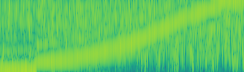
\includegraphics[interpolate=true,width=2.780000in,height=0.810000in]{figures/first_layer-img2.png}}%
\end{pgfscope}%
\begin{pgfscope}%
\pgfsetbuttcap%
\pgfsetroundjoin%
\definecolor{currentfill}{rgb}{0.000000,0.000000,0.000000}%
\pgfsetfillcolor{currentfill}%
\pgfsetlinewidth{0.803000pt}%
\definecolor{currentstroke}{rgb}{0.000000,0.000000,0.000000}%
\pgfsetstrokecolor{currentstroke}%
\pgfsetdash{}{0pt}%
\pgfsys@defobject{currentmarker}{\pgfqpoint{0.000000in}{-0.048611in}}{\pgfqpoint{0.000000in}{0.000000in}}{%
\pgfpathmoveto{\pgfqpoint{0.000000in}{0.000000in}}%
\pgfpathlineto{\pgfqpoint{0.000000in}{-0.048611in}}%
\pgfusepath{stroke,fill}%
}%
\begin{pgfscope}%
\pgfsys@transformshift{0.913219in}{1.661616in}%
\pgfsys@useobject{currentmarker}{}%
\end{pgfscope}%
\end{pgfscope}%
\begin{pgfscope}%
\definecolor{textcolor}{rgb}{0.000000,0.000000,0.000000}%
\pgfsetstrokecolor{textcolor}%
\pgfsetfillcolor{textcolor}%
\pgftext[x=0.913219in,y=1.564393in,,top]{\color{textcolor}\rmfamily\fontsize{10.000000}{12.000000}\selectfont \(\displaystyle {100}\)}%
\end{pgfscope}%
\begin{pgfscope}%
\pgfsetbuttcap%
\pgfsetroundjoin%
\definecolor{currentfill}{rgb}{0.000000,0.000000,0.000000}%
\pgfsetfillcolor{currentfill}%
\pgfsetlinewidth{0.803000pt}%
\definecolor{currentstroke}{rgb}{0.000000,0.000000,0.000000}%
\pgfsetstrokecolor{currentstroke}%
\pgfsetdash{}{0pt}%
\pgfsys@defobject{currentmarker}{\pgfqpoint{0.000000in}{-0.048611in}}{\pgfqpoint{0.000000in}{0.000000in}}{%
\pgfpathmoveto{\pgfqpoint{0.000000in}{0.000000in}}%
\pgfpathlineto{\pgfqpoint{0.000000in}{-0.048611in}}%
\pgfusepath{stroke,fill}%
}%
\begin{pgfscope}%
\pgfsys@transformshift{1.456874in}{1.661616in}%
\pgfsys@useobject{currentmarker}{}%
\end{pgfscope}%
\end{pgfscope}%
\begin{pgfscope}%
\definecolor{textcolor}{rgb}{0.000000,0.000000,0.000000}%
\pgfsetstrokecolor{textcolor}%
\pgfsetfillcolor{textcolor}%
\pgftext[x=1.456874in,y=1.564393in,,top]{\color{textcolor}\rmfamily\fontsize{10.000000}{12.000000}\selectfont \(\displaystyle {200}\)}%
\end{pgfscope}%
\begin{pgfscope}%
\pgfsetbuttcap%
\pgfsetroundjoin%
\definecolor{currentfill}{rgb}{0.000000,0.000000,0.000000}%
\pgfsetfillcolor{currentfill}%
\pgfsetlinewidth{0.803000pt}%
\definecolor{currentstroke}{rgb}{0.000000,0.000000,0.000000}%
\pgfsetstrokecolor{currentstroke}%
\pgfsetdash{}{0pt}%
\pgfsys@defobject{currentmarker}{\pgfqpoint{0.000000in}{-0.048611in}}{\pgfqpoint{0.000000in}{0.000000in}}{%
\pgfpathmoveto{\pgfqpoint{0.000000in}{0.000000in}}%
\pgfpathlineto{\pgfqpoint{0.000000in}{-0.048611in}}%
\pgfusepath{stroke,fill}%
}%
\begin{pgfscope}%
\pgfsys@transformshift{2.000529in}{1.661616in}%
\pgfsys@useobject{currentmarker}{}%
\end{pgfscope}%
\end{pgfscope}%
\begin{pgfscope}%
\definecolor{textcolor}{rgb}{0.000000,0.000000,0.000000}%
\pgfsetstrokecolor{textcolor}%
\pgfsetfillcolor{textcolor}%
\pgftext[x=2.000529in,y=1.564393in,,top]{\color{textcolor}\rmfamily\fontsize{10.000000}{12.000000}\selectfont \(\displaystyle {300}\)}%
\end{pgfscope}%
\begin{pgfscope}%
\pgfsetbuttcap%
\pgfsetroundjoin%
\definecolor{currentfill}{rgb}{0.000000,0.000000,0.000000}%
\pgfsetfillcolor{currentfill}%
\pgfsetlinewidth{0.803000pt}%
\definecolor{currentstroke}{rgb}{0.000000,0.000000,0.000000}%
\pgfsetstrokecolor{currentstroke}%
\pgfsetdash{}{0pt}%
\pgfsys@defobject{currentmarker}{\pgfqpoint{0.000000in}{-0.048611in}}{\pgfqpoint{0.000000in}{0.000000in}}{%
\pgfpathmoveto{\pgfqpoint{0.000000in}{0.000000in}}%
\pgfpathlineto{\pgfqpoint{0.000000in}{-0.048611in}}%
\pgfusepath{stroke,fill}%
}%
\begin{pgfscope}%
\pgfsys@transformshift{2.544184in}{1.661616in}%
\pgfsys@useobject{currentmarker}{}%
\end{pgfscope}%
\end{pgfscope}%
\begin{pgfscope}%
\definecolor{textcolor}{rgb}{0.000000,0.000000,0.000000}%
\pgfsetstrokecolor{textcolor}%
\pgfsetfillcolor{textcolor}%
\pgftext[x=2.544184in,y=1.564393in,,top]{\color{textcolor}\rmfamily\fontsize{10.000000}{12.000000}\selectfont \(\displaystyle {400}\)}%
\end{pgfscope}%
\begin{pgfscope}%
\pgfsetbuttcap%
\pgfsetroundjoin%
\definecolor{currentfill}{rgb}{0.000000,0.000000,0.000000}%
\pgfsetfillcolor{currentfill}%
\pgfsetlinewidth{0.803000pt}%
\definecolor{currentstroke}{rgb}{0.000000,0.000000,0.000000}%
\pgfsetstrokecolor{currentstroke}%
\pgfsetdash{}{0pt}%
\pgfsys@defobject{currentmarker}{\pgfqpoint{0.000000in}{-0.048611in}}{\pgfqpoint{0.000000in}{0.000000in}}{%
\pgfpathmoveto{\pgfqpoint{0.000000in}{0.000000in}}%
\pgfpathlineto{\pgfqpoint{0.000000in}{-0.048611in}}%
\pgfusepath{stroke,fill}%
}%
\begin{pgfscope}%
\pgfsys@transformshift{3.087840in}{1.661616in}%
\pgfsys@useobject{currentmarker}{}%
\end{pgfscope}%
\end{pgfscope}%
\begin{pgfscope}%
\definecolor{textcolor}{rgb}{0.000000,0.000000,0.000000}%
\pgfsetstrokecolor{textcolor}%
\pgfsetfillcolor{textcolor}%
\pgftext[x=3.087840in,y=1.564393in,,top]{\color{textcolor}\rmfamily\fontsize{10.000000}{12.000000}\selectfont \(\displaystyle {500}\)}%
\end{pgfscope}%
\begin{pgfscope}%
\pgfsetbuttcap%
\pgfsetroundjoin%
\definecolor{currentfill}{rgb}{0.000000,0.000000,0.000000}%
\pgfsetfillcolor{currentfill}%
\pgfsetlinewidth{0.803000pt}%
\definecolor{currentstroke}{rgb}{0.000000,0.000000,0.000000}%
\pgfsetstrokecolor{currentstroke}%
\pgfsetdash{}{0pt}%
\pgfsys@defobject{currentmarker}{\pgfqpoint{-0.048611in}{0.000000in}}{\pgfqpoint{-0.000000in}{0.000000in}}{%
\pgfpathmoveto{\pgfqpoint{-0.000000in}{0.000000in}}%
\pgfpathlineto{\pgfqpoint{-0.048611in}{0.000000in}}%
\pgfusepath{stroke,fill}%
}%
\begin{pgfscope}%
\pgfsys@transformshift{0.375000in}{1.661616in}%
\pgfsys@useobject{currentmarker}{}%
\end{pgfscope}%
\end{pgfscope}%
\begin{pgfscope}%
\definecolor{textcolor}{rgb}{0.000000,0.000000,0.000000}%
\pgfsetstrokecolor{textcolor}%
\pgfsetfillcolor{textcolor}%
\pgftext[x=0.208333in, y=1.613390in, left, base]{\color{textcolor}\rmfamily\fontsize{10.000000}{12.000000}\selectfont \(\displaystyle {0}\)}%
\end{pgfscope}%
\begin{pgfscope}%
\pgfsetbuttcap%
\pgfsetroundjoin%
\definecolor{currentfill}{rgb}{0.000000,0.000000,0.000000}%
\pgfsetfillcolor{currentfill}%
\pgfsetlinewidth{0.803000pt}%
\definecolor{currentstroke}{rgb}{0.000000,0.000000,0.000000}%
\pgfsetstrokecolor{currentstroke}%
\pgfsetdash{}{0pt}%
\pgfsys@defobject{currentmarker}{\pgfqpoint{-0.048611in}{0.000000in}}{\pgfqpoint{-0.000000in}{0.000000in}}{%
\pgfpathmoveto{\pgfqpoint{-0.000000in}{0.000000in}}%
\pgfpathlineto{\pgfqpoint{-0.048611in}{0.000000in}}%
\pgfusepath{stroke,fill}%
}%
\begin{pgfscope}%
\pgfsys@transformshift{0.375000in}{2.064183in}%
\pgfsys@useobject{currentmarker}{}%
\end{pgfscope}%
\end{pgfscope}%
\begin{pgfscope}%
\definecolor{textcolor}{rgb}{0.000000,0.000000,0.000000}%
\pgfsetstrokecolor{textcolor}%
\pgfsetfillcolor{textcolor}%
\pgftext[x=0.208333in, y=2.015958in, left, base]{\color{textcolor}\rmfamily\fontsize{10.000000}{12.000000}\selectfont \(\displaystyle {4}\)}%
\end{pgfscope}%
\begin{pgfscope}%
\pgfsetbuttcap%
\pgfsetroundjoin%
\definecolor{currentfill}{rgb}{0.000000,0.000000,0.000000}%
\pgfsetfillcolor{currentfill}%
\pgfsetlinewidth{0.803000pt}%
\definecolor{currentstroke}{rgb}{0.000000,0.000000,0.000000}%
\pgfsetstrokecolor{currentstroke}%
\pgfsetdash{}{0pt}%
\pgfsys@defobject{currentmarker}{\pgfqpoint{-0.048611in}{0.000000in}}{\pgfqpoint{-0.000000in}{0.000000in}}{%
\pgfpathmoveto{\pgfqpoint{-0.000000in}{0.000000in}}%
\pgfpathlineto{\pgfqpoint{-0.048611in}{0.000000in}}%
\pgfusepath{stroke,fill}%
}%
\begin{pgfscope}%
\pgfsys@transformshift{0.375000in}{2.466750in}%
\pgfsys@useobject{currentmarker}{}%
\end{pgfscope}%
\end{pgfscope}%
\begin{pgfscope}%
\definecolor{textcolor}{rgb}{0.000000,0.000000,0.000000}%
\pgfsetstrokecolor{textcolor}%
\pgfsetfillcolor{textcolor}%
\pgftext[x=0.208333in, y=2.418525in, left, base]{\color{textcolor}\rmfamily\fontsize{10.000000}{12.000000}\selectfont \(\displaystyle {8}\)}%
\end{pgfscope}%
\begin{pgfscope}%
\definecolor{textcolor}{rgb}{0.000000,0.000000,0.000000}%
\pgfsetstrokecolor{textcolor}%
\pgfsetfillcolor{textcolor}%
\pgftext[x=0.152778in,y=2.064183in,,bottom,rotate=90.000000]{\color{textcolor}\rmfamily\fontsize{10.000000}{12.000000}\selectfont Frequency [\si{\kilo\hertz}]}%
\end{pgfscope}%
\begin{pgfscope}%
\pgfsetrectcap%
\pgfsetmiterjoin%
\pgfsetlinewidth{0.803000pt}%
\definecolor{currentstroke}{rgb}{0.000000,0.000000,0.000000}%
\pgfsetstrokecolor{currentstroke}%
\pgfsetdash{}{0pt}%
\pgfpathmoveto{\pgfqpoint{0.375000in}{1.661616in}}%
\pgfpathlineto{\pgfqpoint{0.375000in}{2.466750in}}%
\pgfusepath{stroke}%
\end{pgfscope}%
\begin{pgfscope}%
\pgfsetrectcap%
\pgfsetmiterjoin%
\pgfsetlinewidth{0.803000pt}%
\definecolor{currentstroke}{rgb}{0.000000,0.000000,0.000000}%
\pgfsetstrokecolor{currentstroke}%
\pgfsetdash{}{0pt}%
\pgfpathmoveto{\pgfqpoint{3.153078in}{1.661616in}}%
\pgfpathlineto{\pgfqpoint{3.153078in}{2.466750in}}%
\pgfusepath{stroke}%
\end{pgfscope}%
\begin{pgfscope}%
\pgfsetrectcap%
\pgfsetmiterjoin%
\pgfsetlinewidth{0.803000pt}%
\definecolor{currentstroke}{rgb}{0.000000,0.000000,0.000000}%
\pgfsetstrokecolor{currentstroke}%
\pgfsetdash{}{0pt}%
\pgfpathmoveto{\pgfqpoint{0.375000in}{1.661616in}}%
\pgfpathlineto{\pgfqpoint{3.153078in}{1.661616in}}%
\pgfusepath{stroke}%
\end{pgfscope}%
\begin{pgfscope}%
\pgfsetrectcap%
\pgfsetmiterjoin%
\pgfsetlinewidth{0.803000pt}%
\definecolor{currentstroke}{rgb}{0.000000,0.000000,0.000000}%
\pgfsetstrokecolor{currentstroke}%
\pgfsetdash{}{0pt}%
\pgfpathmoveto{\pgfqpoint{0.375000in}{2.466750in}}%
\pgfpathlineto{\pgfqpoint{3.153078in}{2.466750in}}%
\pgfusepath{stroke}%
\end{pgfscope}%
\begin{pgfscope}%
\definecolor{textcolor}{rgb}{0.000000,0.000000,0.000000}%
\pgfsetstrokecolor{textcolor}%
\pgfsetfillcolor{textcolor}%
\pgftext[x=1.764039in,y=2.550083in,,base]{\color{textcolor}\rmfamily\fontsize{12.000000}{14.400000}\selectfont (c) wav2vec 2.0 FE}%
\end{pgfscope}%
\begin{pgfscope}%
\pgfsetbuttcap%
\pgfsetmiterjoin%
\definecolor{currentfill}{rgb}{1.000000,1.000000,1.000000}%
\pgfsetfillcolor{currentfill}%
\pgfsetlinewidth{0.000000pt}%
\definecolor{currentstroke}{rgb}{0.000000,0.000000,0.000000}%
\pgfsetstrokecolor{currentstroke}%
\pgfsetstrokeopacity{0.000000}%
\pgfsetdash{}{0pt}%
\pgfpathmoveto{\pgfqpoint{3.403079in}{1.661616in}}%
\pgfpathlineto{\pgfqpoint{6.181157in}{1.661616in}}%
\pgfpathlineto{\pgfqpoint{6.181157in}{2.466750in}}%
\pgfpathlineto{\pgfqpoint{3.403079in}{2.466750in}}%
\pgfpathlineto{\pgfqpoint{3.403079in}{1.661616in}}%
\pgfpathclose%
\pgfusepath{fill}%
\end{pgfscope}%
\begin{pgfscope}%
\pgfpathrectangle{\pgfqpoint{3.403079in}{1.661616in}}{\pgfqpoint{2.778078in}{0.805134in}}%
\pgfusepath{clip}%
\pgfsys@transformshift{3.403079in}{1.661616in}%
\pgftext[left,bottom]{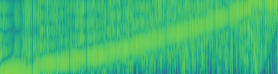
\includegraphics[interpolate=true,width=2.780000in,height=0.810000in]{figures/first_layer-img3.png}}%
\end{pgfscope}%
\begin{pgfscope}%
\pgfsetbuttcap%
\pgfsetroundjoin%
\definecolor{currentfill}{rgb}{0.000000,0.000000,0.000000}%
\pgfsetfillcolor{currentfill}%
\pgfsetlinewidth{0.803000pt}%
\definecolor{currentstroke}{rgb}{0.000000,0.000000,0.000000}%
\pgfsetstrokecolor{currentstroke}%
\pgfsetdash{}{0pt}%
\pgfsys@defobject{currentmarker}{\pgfqpoint{0.000000in}{-0.048611in}}{\pgfqpoint{0.000000in}{0.000000in}}{%
\pgfpathmoveto{\pgfqpoint{0.000000in}{0.000000in}}%
\pgfpathlineto{\pgfqpoint{0.000000in}{-0.048611in}}%
\pgfusepath{stroke,fill}%
}%
\begin{pgfscope}%
\pgfsys@transformshift{3.941297in}{1.661616in}%
\pgfsys@useobject{currentmarker}{}%
\end{pgfscope}%
\end{pgfscope}%
\begin{pgfscope}%
\definecolor{textcolor}{rgb}{0.000000,0.000000,0.000000}%
\pgfsetstrokecolor{textcolor}%
\pgfsetfillcolor{textcolor}%
\pgftext[x=3.941297in,y=1.564393in,,top]{\color{textcolor}\rmfamily\fontsize{10.000000}{12.000000}\selectfont \(\displaystyle {100}\)}%
\end{pgfscope}%
\begin{pgfscope}%
\pgfsetbuttcap%
\pgfsetroundjoin%
\definecolor{currentfill}{rgb}{0.000000,0.000000,0.000000}%
\pgfsetfillcolor{currentfill}%
\pgfsetlinewidth{0.803000pt}%
\definecolor{currentstroke}{rgb}{0.000000,0.000000,0.000000}%
\pgfsetstrokecolor{currentstroke}%
\pgfsetdash{}{0pt}%
\pgfsys@defobject{currentmarker}{\pgfqpoint{0.000000in}{-0.048611in}}{\pgfqpoint{0.000000in}{0.000000in}}{%
\pgfpathmoveto{\pgfqpoint{0.000000in}{0.000000in}}%
\pgfpathlineto{\pgfqpoint{0.000000in}{-0.048611in}}%
\pgfusepath{stroke,fill}%
}%
\begin{pgfscope}%
\pgfsys@transformshift{4.484953in}{1.661616in}%
\pgfsys@useobject{currentmarker}{}%
\end{pgfscope}%
\end{pgfscope}%
\begin{pgfscope}%
\definecolor{textcolor}{rgb}{0.000000,0.000000,0.000000}%
\pgfsetstrokecolor{textcolor}%
\pgfsetfillcolor{textcolor}%
\pgftext[x=4.484953in,y=1.564393in,,top]{\color{textcolor}\rmfamily\fontsize{10.000000}{12.000000}\selectfont \(\displaystyle {200}\)}%
\end{pgfscope}%
\begin{pgfscope}%
\pgfsetbuttcap%
\pgfsetroundjoin%
\definecolor{currentfill}{rgb}{0.000000,0.000000,0.000000}%
\pgfsetfillcolor{currentfill}%
\pgfsetlinewidth{0.803000pt}%
\definecolor{currentstroke}{rgb}{0.000000,0.000000,0.000000}%
\pgfsetstrokecolor{currentstroke}%
\pgfsetdash{}{0pt}%
\pgfsys@defobject{currentmarker}{\pgfqpoint{0.000000in}{-0.048611in}}{\pgfqpoint{0.000000in}{0.000000in}}{%
\pgfpathmoveto{\pgfqpoint{0.000000in}{0.000000in}}%
\pgfpathlineto{\pgfqpoint{0.000000in}{-0.048611in}}%
\pgfusepath{stroke,fill}%
}%
\begin{pgfscope}%
\pgfsys@transformshift{5.028608in}{1.661616in}%
\pgfsys@useobject{currentmarker}{}%
\end{pgfscope}%
\end{pgfscope}%
\begin{pgfscope}%
\definecolor{textcolor}{rgb}{0.000000,0.000000,0.000000}%
\pgfsetstrokecolor{textcolor}%
\pgfsetfillcolor{textcolor}%
\pgftext[x=5.028608in,y=1.564393in,,top]{\color{textcolor}\rmfamily\fontsize{10.000000}{12.000000}\selectfont \(\displaystyle {300}\)}%
\end{pgfscope}%
\begin{pgfscope}%
\pgfsetbuttcap%
\pgfsetroundjoin%
\definecolor{currentfill}{rgb}{0.000000,0.000000,0.000000}%
\pgfsetfillcolor{currentfill}%
\pgfsetlinewidth{0.803000pt}%
\definecolor{currentstroke}{rgb}{0.000000,0.000000,0.000000}%
\pgfsetstrokecolor{currentstroke}%
\pgfsetdash{}{0pt}%
\pgfsys@defobject{currentmarker}{\pgfqpoint{0.000000in}{-0.048611in}}{\pgfqpoint{0.000000in}{0.000000in}}{%
\pgfpathmoveto{\pgfqpoint{0.000000in}{0.000000in}}%
\pgfpathlineto{\pgfqpoint{0.000000in}{-0.048611in}}%
\pgfusepath{stroke,fill}%
}%
\begin{pgfscope}%
\pgfsys@transformshift{5.572263in}{1.661616in}%
\pgfsys@useobject{currentmarker}{}%
\end{pgfscope}%
\end{pgfscope}%
\begin{pgfscope}%
\definecolor{textcolor}{rgb}{0.000000,0.000000,0.000000}%
\pgfsetstrokecolor{textcolor}%
\pgfsetfillcolor{textcolor}%
\pgftext[x=5.572263in,y=1.564393in,,top]{\color{textcolor}\rmfamily\fontsize{10.000000}{12.000000}\selectfont \(\displaystyle {400}\)}%
\end{pgfscope}%
\begin{pgfscope}%
\pgfsetbuttcap%
\pgfsetroundjoin%
\definecolor{currentfill}{rgb}{0.000000,0.000000,0.000000}%
\pgfsetfillcolor{currentfill}%
\pgfsetlinewidth{0.803000pt}%
\definecolor{currentstroke}{rgb}{0.000000,0.000000,0.000000}%
\pgfsetstrokecolor{currentstroke}%
\pgfsetdash{}{0pt}%
\pgfsys@defobject{currentmarker}{\pgfqpoint{0.000000in}{-0.048611in}}{\pgfqpoint{0.000000in}{0.000000in}}{%
\pgfpathmoveto{\pgfqpoint{0.000000in}{0.000000in}}%
\pgfpathlineto{\pgfqpoint{0.000000in}{-0.048611in}}%
\pgfusepath{stroke,fill}%
}%
\begin{pgfscope}%
\pgfsys@transformshift{6.115918in}{1.661616in}%
\pgfsys@useobject{currentmarker}{}%
\end{pgfscope}%
\end{pgfscope}%
\begin{pgfscope}%
\definecolor{textcolor}{rgb}{0.000000,0.000000,0.000000}%
\pgfsetstrokecolor{textcolor}%
\pgfsetfillcolor{textcolor}%
\pgftext[x=6.115918in,y=1.564393in,,top]{\color{textcolor}\rmfamily\fontsize{10.000000}{12.000000}\selectfont \(\displaystyle {500}\)}%
\end{pgfscope}%
\begin{pgfscope}%
\pgfsetbuttcap%
\pgfsetroundjoin%
\definecolor{currentfill}{rgb}{0.000000,0.000000,0.000000}%
\pgfsetfillcolor{currentfill}%
\pgfsetlinewidth{0.803000pt}%
\definecolor{currentstroke}{rgb}{0.000000,0.000000,0.000000}%
\pgfsetstrokecolor{currentstroke}%
\pgfsetdash{}{0pt}%
\pgfsys@defobject{currentmarker}{\pgfqpoint{-0.048611in}{0.000000in}}{\pgfqpoint{-0.000000in}{0.000000in}}{%
\pgfpathmoveto{\pgfqpoint{-0.000000in}{0.000000in}}%
\pgfpathlineto{\pgfqpoint{-0.048611in}{0.000000in}}%
\pgfusepath{stroke,fill}%
}%
\begin{pgfscope}%
\pgfsys@transformshift{3.403079in}{1.661616in}%
\pgfsys@useobject{currentmarker}{}%
\end{pgfscope}%
\end{pgfscope}%
\begin{pgfscope}%
\definecolor{textcolor}{rgb}{0.000000,0.000000,0.000000}%
\pgfsetstrokecolor{textcolor}%
\pgfsetfillcolor{textcolor}%
\pgftext[x=3.236412in, y=1.613390in, left, base]{\color{textcolor}\rmfamily\fontsize{10.000000}{12.000000}\selectfont \(\displaystyle {0}\)}%
\end{pgfscope}%
\begin{pgfscope}%
\pgfsetbuttcap%
\pgfsetroundjoin%
\definecolor{currentfill}{rgb}{0.000000,0.000000,0.000000}%
\pgfsetfillcolor{currentfill}%
\pgfsetlinewidth{0.803000pt}%
\definecolor{currentstroke}{rgb}{0.000000,0.000000,0.000000}%
\pgfsetstrokecolor{currentstroke}%
\pgfsetdash{}{0pt}%
\pgfsys@defobject{currentmarker}{\pgfqpoint{-0.048611in}{0.000000in}}{\pgfqpoint{-0.000000in}{0.000000in}}{%
\pgfpathmoveto{\pgfqpoint{-0.000000in}{0.000000in}}%
\pgfpathlineto{\pgfqpoint{-0.048611in}{0.000000in}}%
\pgfusepath{stroke,fill}%
}%
\begin{pgfscope}%
\pgfsys@transformshift{3.403079in}{2.064183in}%
\pgfsys@useobject{currentmarker}{}%
\end{pgfscope}%
\end{pgfscope}%
\begin{pgfscope}%
\definecolor{textcolor}{rgb}{0.000000,0.000000,0.000000}%
\pgfsetstrokecolor{textcolor}%
\pgfsetfillcolor{textcolor}%
\pgftext[x=3.236412in, y=2.015958in, left, base]{\color{textcolor}\rmfamily\fontsize{10.000000}{12.000000}\selectfont \(\displaystyle {4}\)}%
\end{pgfscope}%
\begin{pgfscope}%
\pgfsetbuttcap%
\pgfsetroundjoin%
\definecolor{currentfill}{rgb}{0.000000,0.000000,0.000000}%
\pgfsetfillcolor{currentfill}%
\pgfsetlinewidth{0.803000pt}%
\definecolor{currentstroke}{rgb}{0.000000,0.000000,0.000000}%
\pgfsetstrokecolor{currentstroke}%
\pgfsetdash{}{0pt}%
\pgfsys@defobject{currentmarker}{\pgfqpoint{-0.048611in}{0.000000in}}{\pgfqpoint{-0.000000in}{0.000000in}}{%
\pgfpathmoveto{\pgfqpoint{-0.000000in}{0.000000in}}%
\pgfpathlineto{\pgfqpoint{-0.048611in}{0.000000in}}%
\pgfusepath{stroke,fill}%
}%
\begin{pgfscope}%
\pgfsys@transformshift{3.403079in}{2.466750in}%
\pgfsys@useobject{currentmarker}{}%
\end{pgfscope}%
\end{pgfscope}%
\begin{pgfscope}%
\definecolor{textcolor}{rgb}{0.000000,0.000000,0.000000}%
\pgfsetstrokecolor{textcolor}%
\pgfsetfillcolor{textcolor}%
\pgftext[x=3.236412in, y=2.418525in, left, base]{\color{textcolor}\rmfamily\fontsize{10.000000}{12.000000}\selectfont \(\displaystyle {8}\)}%
\end{pgfscope}%
\begin{pgfscope}%
\pgfsetrectcap%
\pgfsetmiterjoin%
\pgfsetlinewidth{0.803000pt}%
\definecolor{currentstroke}{rgb}{0.000000,0.000000,0.000000}%
\pgfsetstrokecolor{currentstroke}%
\pgfsetdash{}{0pt}%
\pgfpathmoveto{\pgfqpoint{3.403079in}{1.661616in}}%
\pgfpathlineto{\pgfqpoint{3.403079in}{2.466750in}}%
\pgfusepath{stroke}%
\end{pgfscope}%
\begin{pgfscope}%
\pgfsetrectcap%
\pgfsetmiterjoin%
\pgfsetlinewidth{0.803000pt}%
\definecolor{currentstroke}{rgb}{0.000000,0.000000,0.000000}%
\pgfsetstrokecolor{currentstroke}%
\pgfsetdash{}{0pt}%
\pgfpathmoveto{\pgfqpoint{6.181157in}{1.661616in}}%
\pgfpathlineto{\pgfqpoint{6.181157in}{2.466750in}}%
\pgfusepath{stroke}%
\end{pgfscope}%
\begin{pgfscope}%
\pgfsetrectcap%
\pgfsetmiterjoin%
\pgfsetlinewidth{0.803000pt}%
\definecolor{currentstroke}{rgb}{0.000000,0.000000,0.000000}%
\pgfsetstrokecolor{currentstroke}%
\pgfsetdash{}{0pt}%
\pgfpathmoveto{\pgfqpoint{3.403079in}{1.661616in}}%
\pgfpathlineto{\pgfqpoint{6.181157in}{1.661616in}}%
\pgfusepath{stroke}%
\end{pgfscope}%
\begin{pgfscope}%
\pgfsetrectcap%
\pgfsetmiterjoin%
\pgfsetlinewidth{0.803000pt}%
\definecolor{currentstroke}{rgb}{0.000000,0.000000,0.000000}%
\pgfsetstrokecolor{currentstroke}%
\pgfsetdash{}{0pt}%
\pgfpathmoveto{\pgfqpoint{3.403079in}{2.466750in}}%
\pgfpathlineto{\pgfqpoint{6.181157in}{2.466750in}}%
\pgfusepath{stroke}%
\end{pgfscope}%
\begin{pgfscope}%
\definecolor{textcolor}{rgb}{0.000000,0.000000,0.000000}%
\pgfsetstrokecolor{textcolor}%
\pgfsetfillcolor{textcolor}%
\pgftext[x=4.792118in,y=2.550083in,,base]{\color{textcolor}\rmfamily\fontsize{12.000000}{14.400000}\selectfont (d) wav2vec 2.0 FE (pre-training)}%
\end{pgfscope}%
\begin{pgfscope}%
\pgfsetbuttcap%
\pgfsetmiterjoin%
\definecolor{currentfill}{rgb}{1.000000,1.000000,1.000000}%
\pgfsetfillcolor{currentfill}%
\pgfsetlinewidth{0.000000pt}%
\definecolor{currentstroke}{rgb}{0.000000,0.000000,0.000000}%
\pgfsetstrokecolor{currentstroke}%
\pgfsetstrokeopacity{0.000000}%
\pgfsetdash{}{0pt}%
\pgfpathmoveto{\pgfqpoint{0.375000in}{0.413580in}}%
\pgfpathlineto{\pgfqpoint{3.153078in}{0.413580in}}%
\pgfpathlineto{\pgfqpoint{3.153078in}{1.218714in}}%
\pgfpathlineto{\pgfqpoint{0.375000in}{1.218714in}}%
\pgfpathlineto{\pgfqpoint{0.375000in}{0.413580in}}%
\pgfpathclose%
\pgfusepath{fill}%
\end{pgfscope}%
\begin{pgfscope}%
\pgfpathrectangle{\pgfqpoint{0.375000in}{0.413580in}}{\pgfqpoint{2.778078in}{0.805134in}}%
\pgfusepath{clip}%
\pgfsys@transformshift{0.375000in}{0.413580in}%
\pgftext[left,bottom]{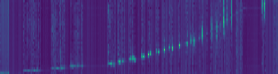
\includegraphics[interpolate=true,width=2.780000in,height=0.810000in]{figures/first_layer-img4.png}}%
\end{pgfscope}%
\begin{pgfscope}%
\pgfsetbuttcap%
\pgfsetroundjoin%
\definecolor{currentfill}{rgb}{0.000000,0.000000,0.000000}%
\pgfsetfillcolor{currentfill}%
\pgfsetlinewidth{0.803000pt}%
\definecolor{currentstroke}{rgb}{0.000000,0.000000,0.000000}%
\pgfsetstrokecolor{currentstroke}%
\pgfsetdash{}{0pt}%
\pgfsys@defobject{currentmarker}{\pgfqpoint{0.000000in}{-0.048611in}}{\pgfqpoint{0.000000in}{0.000000in}}{%
\pgfpathmoveto{\pgfqpoint{0.000000in}{0.000000in}}%
\pgfpathlineto{\pgfqpoint{0.000000in}{-0.048611in}}%
\pgfusepath{stroke,fill}%
}%
\begin{pgfscope}%
\pgfsys@transformshift{1.113101in}{0.413580in}%
\pgfsys@useobject{currentmarker}{}%
\end{pgfscope}%
\end{pgfscope}%
\begin{pgfscope}%
\definecolor{textcolor}{rgb}{0.000000,0.000000,0.000000}%
\pgfsetstrokecolor{textcolor}%
\pgfsetfillcolor{textcolor}%
\pgftext[x=1.113101in,y=0.316358in,,top]{\color{textcolor}\rmfamily\fontsize{10.000000}{12.000000}\selectfont \(\displaystyle {200}\)}%
\end{pgfscope}%
\begin{pgfscope}%
\pgfsetbuttcap%
\pgfsetroundjoin%
\definecolor{currentfill}{rgb}{0.000000,0.000000,0.000000}%
\pgfsetfillcolor{currentfill}%
\pgfsetlinewidth{0.803000pt}%
\definecolor{currentstroke}{rgb}{0.000000,0.000000,0.000000}%
\pgfsetstrokecolor{currentstroke}%
\pgfsetdash{}{0pt}%
\pgfsys@defobject{currentmarker}{\pgfqpoint{0.000000in}{-0.048611in}}{\pgfqpoint{0.000000in}{0.000000in}}{%
\pgfpathmoveto{\pgfqpoint{0.000000in}{0.000000in}}%
\pgfpathlineto{\pgfqpoint{0.000000in}{-0.048611in}}%
\pgfusepath{stroke,fill}%
}%
\begin{pgfscope}%
\pgfsys@transformshift{1.854911in}{0.413580in}%
\pgfsys@useobject{currentmarker}{}%
\end{pgfscope}%
\end{pgfscope}%
\begin{pgfscope}%
\definecolor{textcolor}{rgb}{0.000000,0.000000,0.000000}%
\pgfsetstrokecolor{textcolor}%
\pgfsetfillcolor{textcolor}%
\pgftext[x=1.854911in,y=0.316358in,,top]{\color{textcolor}\rmfamily\fontsize{10.000000}{12.000000}\selectfont \(\displaystyle {400}\)}%
\end{pgfscope}%
\begin{pgfscope}%
\pgfsetbuttcap%
\pgfsetroundjoin%
\definecolor{currentfill}{rgb}{0.000000,0.000000,0.000000}%
\pgfsetfillcolor{currentfill}%
\pgfsetlinewidth{0.803000pt}%
\definecolor{currentstroke}{rgb}{0.000000,0.000000,0.000000}%
\pgfsetstrokecolor{currentstroke}%
\pgfsetdash{}{0pt}%
\pgfsys@defobject{currentmarker}{\pgfqpoint{0.000000in}{-0.048611in}}{\pgfqpoint{0.000000in}{0.000000in}}{%
\pgfpathmoveto{\pgfqpoint{0.000000in}{0.000000in}}%
\pgfpathlineto{\pgfqpoint{0.000000in}{-0.048611in}}%
\pgfusepath{stroke,fill}%
}%
\begin{pgfscope}%
\pgfsys@transformshift{2.596721in}{0.413580in}%
\pgfsys@useobject{currentmarker}{}%
\end{pgfscope}%
\end{pgfscope}%
\begin{pgfscope}%
\definecolor{textcolor}{rgb}{0.000000,0.000000,0.000000}%
\pgfsetstrokecolor{textcolor}%
\pgfsetfillcolor{textcolor}%
\pgftext[x=2.596721in,y=0.316358in,,top]{\color{textcolor}\rmfamily\fontsize{10.000000}{12.000000}\selectfont \(\displaystyle {600}\)}%
\end{pgfscope}%
\begin{pgfscope}%
\definecolor{textcolor}{rgb}{0.000000,0.000000,0.000000}%
\pgfsetstrokecolor{textcolor}%
\pgfsetfillcolor{textcolor}%
\pgftext[x=1.764039in,y=0.137346in,,top]{\color{textcolor}\rmfamily\fontsize{10.000000}{12.000000}\selectfont Filter index}%
\end{pgfscope}%
\begin{pgfscope}%
\pgfsetbuttcap%
\pgfsetroundjoin%
\definecolor{currentfill}{rgb}{0.000000,0.000000,0.000000}%
\pgfsetfillcolor{currentfill}%
\pgfsetlinewidth{0.803000pt}%
\definecolor{currentstroke}{rgb}{0.000000,0.000000,0.000000}%
\pgfsetstrokecolor{currentstroke}%
\pgfsetdash{}{0pt}%
\pgfsys@defobject{currentmarker}{\pgfqpoint{-0.048611in}{0.000000in}}{\pgfqpoint{-0.000000in}{0.000000in}}{%
\pgfpathmoveto{\pgfqpoint{-0.000000in}{0.000000in}}%
\pgfpathlineto{\pgfqpoint{-0.048611in}{0.000000in}}%
\pgfusepath{stroke,fill}%
}%
\begin{pgfscope}%
\pgfsys@transformshift{0.375000in}{0.413580in}%
\pgfsys@useobject{currentmarker}{}%
\end{pgfscope}%
\end{pgfscope}%
\begin{pgfscope}%
\definecolor{textcolor}{rgb}{0.000000,0.000000,0.000000}%
\pgfsetstrokecolor{textcolor}%
\pgfsetfillcolor{textcolor}%
\pgftext[x=0.208333in, y=0.365355in, left, base]{\color{textcolor}\rmfamily\fontsize{10.000000}{12.000000}\selectfont \(\displaystyle {0}\)}%
\end{pgfscope}%
\begin{pgfscope}%
\pgfsetbuttcap%
\pgfsetroundjoin%
\definecolor{currentfill}{rgb}{0.000000,0.000000,0.000000}%
\pgfsetfillcolor{currentfill}%
\pgfsetlinewidth{0.803000pt}%
\definecolor{currentstroke}{rgb}{0.000000,0.000000,0.000000}%
\pgfsetstrokecolor{currentstroke}%
\pgfsetdash{}{0pt}%
\pgfsys@defobject{currentmarker}{\pgfqpoint{-0.048611in}{0.000000in}}{\pgfqpoint{-0.000000in}{0.000000in}}{%
\pgfpathmoveto{\pgfqpoint{-0.000000in}{0.000000in}}%
\pgfpathlineto{\pgfqpoint{-0.048611in}{0.000000in}}%
\pgfusepath{stroke,fill}%
}%
\begin{pgfscope}%
\pgfsys@transformshift{0.375000in}{0.816147in}%
\pgfsys@useobject{currentmarker}{}%
\end{pgfscope}%
\end{pgfscope}%
\begin{pgfscope}%
\definecolor{textcolor}{rgb}{0.000000,0.000000,0.000000}%
\pgfsetstrokecolor{textcolor}%
\pgfsetfillcolor{textcolor}%
\pgftext[x=0.208333in, y=0.767922in, left, base]{\color{textcolor}\rmfamily\fontsize{10.000000}{12.000000}\selectfont \(\displaystyle {4}\)}%
\end{pgfscope}%
\begin{pgfscope}%
\pgfsetbuttcap%
\pgfsetroundjoin%
\definecolor{currentfill}{rgb}{0.000000,0.000000,0.000000}%
\pgfsetfillcolor{currentfill}%
\pgfsetlinewidth{0.803000pt}%
\definecolor{currentstroke}{rgb}{0.000000,0.000000,0.000000}%
\pgfsetstrokecolor{currentstroke}%
\pgfsetdash{}{0pt}%
\pgfsys@defobject{currentmarker}{\pgfqpoint{-0.048611in}{0.000000in}}{\pgfqpoint{-0.000000in}{0.000000in}}{%
\pgfpathmoveto{\pgfqpoint{-0.000000in}{0.000000in}}%
\pgfpathlineto{\pgfqpoint{-0.048611in}{0.000000in}}%
\pgfusepath{stroke,fill}%
}%
\begin{pgfscope}%
\pgfsys@transformshift{0.375000in}{1.218714in}%
\pgfsys@useobject{currentmarker}{}%
\end{pgfscope}%
\end{pgfscope}%
\begin{pgfscope}%
\definecolor{textcolor}{rgb}{0.000000,0.000000,0.000000}%
\pgfsetstrokecolor{textcolor}%
\pgfsetfillcolor{textcolor}%
\pgftext[x=0.208333in, y=1.170489in, left, base]{\color{textcolor}\rmfamily\fontsize{10.000000}{12.000000}\selectfont \(\displaystyle {8}\)}%
\end{pgfscope}%
\begin{pgfscope}%
\definecolor{textcolor}{rgb}{0.000000,0.000000,0.000000}%
\pgfsetstrokecolor{textcolor}%
\pgfsetfillcolor{textcolor}%
\pgftext[x=0.152778in,y=0.816147in,,bottom,rotate=90.000000]{\color{textcolor}\rmfamily\fontsize{10.000000}{12.000000}\selectfont Frequency [\si{\kilo\hertz}]}%
\end{pgfscope}%
\begin{pgfscope}%
\pgfsetrectcap%
\pgfsetmiterjoin%
\pgfsetlinewidth{0.803000pt}%
\definecolor{currentstroke}{rgb}{0.000000,0.000000,0.000000}%
\pgfsetstrokecolor{currentstroke}%
\pgfsetdash{}{0pt}%
\pgfpathmoveto{\pgfqpoint{0.375000in}{0.413580in}}%
\pgfpathlineto{\pgfqpoint{0.375000in}{1.218714in}}%
\pgfusepath{stroke}%
\end{pgfscope}%
\begin{pgfscope}%
\pgfsetrectcap%
\pgfsetmiterjoin%
\pgfsetlinewidth{0.803000pt}%
\definecolor{currentstroke}{rgb}{0.000000,0.000000,0.000000}%
\pgfsetstrokecolor{currentstroke}%
\pgfsetdash{}{0pt}%
\pgfpathmoveto{\pgfqpoint{3.153078in}{0.413580in}}%
\pgfpathlineto{\pgfqpoint{3.153078in}{1.218714in}}%
\pgfusepath{stroke}%
\end{pgfscope}%
\begin{pgfscope}%
\pgfsetrectcap%
\pgfsetmiterjoin%
\pgfsetlinewidth{0.803000pt}%
\definecolor{currentstroke}{rgb}{0.000000,0.000000,0.000000}%
\pgfsetstrokecolor{currentstroke}%
\pgfsetdash{}{0pt}%
\pgfpathmoveto{\pgfqpoint{0.375000in}{0.413580in}}%
\pgfpathlineto{\pgfqpoint{3.153078in}{0.413580in}}%
\pgfusepath{stroke}%
\end{pgfscope}%
\begin{pgfscope}%
\pgfsetrectcap%
\pgfsetmiterjoin%
\pgfsetlinewidth{0.803000pt}%
\definecolor{currentstroke}{rgb}{0.000000,0.000000,0.000000}%
\pgfsetstrokecolor{currentstroke}%
\pgfsetdash{}{0pt}%
\pgfpathmoveto{\pgfqpoint{0.375000in}{1.218714in}}%
\pgfpathlineto{\pgfqpoint{3.153078in}{1.218714in}}%
\pgfusepath{stroke}%
\end{pgfscope}%
\begin{pgfscope}%
\definecolor{textcolor}{rgb}{0.000000,0.000000,0.000000}%
\pgfsetstrokecolor{textcolor}%
\pgfsetfillcolor{textcolor}%
\pgftext[x=1.764039in,y=1.302048in,,base]{\color{textcolor}\rmfamily\fontsize{12.000000}{14.400000}\selectfont (e) SC}%
\end{pgfscope}%
\begin{pgfscope}%
\pgfsetbuttcap%
\pgfsetmiterjoin%
\definecolor{currentfill}{rgb}{1.000000,1.000000,1.000000}%
\pgfsetfillcolor{currentfill}%
\pgfsetlinewidth{0.000000pt}%
\definecolor{currentstroke}{rgb}{0.000000,0.000000,0.000000}%
\pgfsetstrokecolor{currentstroke}%
\pgfsetstrokeopacity{0.000000}%
\pgfsetdash{}{0pt}%
\pgfpathmoveto{\pgfqpoint{3.403079in}{0.413580in}}%
\pgfpathlineto{\pgfqpoint{6.181157in}{0.413580in}}%
\pgfpathlineto{\pgfqpoint{6.181157in}{1.218714in}}%
\pgfpathlineto{\pgfqpoint{3.403079in}{1.218714in}}%
\pgfpathlineto{\pgfqpoint{3.403079in}{0.413580in}}%
\pgfpathclose%
\pgfusepath{fill}%
\end{pgfscope}%
\begin{pgfscope}%
\pgfpathrectangle{\pgfqpoint{3.403079in}{0.413580in}}{\pgfqpoint{2.778078in}{0.805134in}}%
\pgfusepath{clip}%
\pgfsys@transformshift{3.403079in}{0.413580in}%
\pgftext[left,bottom]{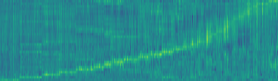
\includegraphics[interpolate=true,width=2.780000in,height=0.810000in]{figures/first_layer-img5.png}}%
\end{pgfscope}%
\begin{pgfscope}%
\pgfsetbuttcap%
\pgfsetroundjoin%
\definecolor{currentfill}{rgb}{0.000000,0.000000,0.000000}%
\pgfsetfillcolor{currentfill}%
\pgfsetlinewidth{0.803000pt}%
\definecolor{currentstroke}{rgb}{0.000000,0.000000,0.000000}%
\pgfsetstrokecolor{currentstroke}%
\pgfsetdash{}{0pt}%
\pgfsys@defobject{currentmarker}{\pgfqpoint{0.000000in}{-0.048611in}}{\pgfqpoint{0.000000in}{0.000000in}}{%
\pgfpathmoveto{\pgfqpoint{0.000000in}{0.000000in}}%
\pgfpathlineto{\pgfqpoint{0.000000in}{-0.048611in}}%
\pgfusepath{stroke,fill}%
}%
\begin{pgfscope}%
\pgfsys@transformshift{4.123858in}{0.413580in}%
\pgfsys@useobject{currentmarker}{}%
\end{pgfscope}%
\end{pgfscope}%
\begin{pgfscope}%
\definecolor{textcolor}{rgb}{0.000000,0.000000,0.000000}%
\pgfsetstrokecolor{textcolor}%
\pgfsetfillcolor{textcolor}%
\pgftext[x=4.123858in,y=0.316358in,,top]{\color{textcolor}\rmfamily\fontsize{10.000000}{12.000000}\selectfont \(\displaystyle {200}\)}%
\end{pgfscope}%
\begin{pgfscope}%
\pgfsetbuttcap%
\pgfsetroundjoin%
\definecolor{currentfill}{rgb}{0.000000,0.000000,0.000000}%
\pgfsetfillcolor{currentfill}%
\pgfsetlinewidth{0.803000pt}%
\definecolor{currentstroke}{rgb}{0.000000,0.000000,0.000000}%
\pgfsetstrokecolor{currentstroke}%
\pgfsetdash{}{0pt}%
\pgfsys@defobject{currentmarker}{\pgfqpoint{0.000000in}{-0.048611in}}{\pgfqpoint{0.000000in}{0.000000in}}{%
\pgfpathmoveto{\pgfqpoint{0.000000in}{0.000000in}}%
\pgfpathlineto{\pgfqpoint{0.000000in}{-0.048611in}}%
\pgfusepath{stroke,fill}%
}%
\begin{pgfscope}%
\pgfsys@transformshift{4.848259in}{0.413580in}%
\pgfsys@useobject{currentmarker}{}%
\end{pgfscope}%
\end{pgfscope}%
\begin{pgfscope}%
\definecolor{textcolor}{rgb}{0.000000,0.000000,0.000000}%
\pgfsetstrokecolor{textcolor}%
\pgfsetfillcolor{textcolor}%
\pgftext[x=4.848259in,y=0.316358in,,top]{\color{textcolor}\rmfamily\fontsize{10.000000}{12.000000}\selectfont \(\displaystyle {400}\)}%
\end{pgfscope}%
\begin{pgfscope}%
\pgfsetbuttcap%
\pgfsetroundjoin%
\definecolor{currentfill}{rgb}{0.000000,0.000000,0.000000}%
\pgfsetfillcolor{currentfill}%
\pgfsetlinewidth{0.803000pt}%
\definecolor{currentstroke}{rgb}{0.000000,0.000000,0.000000}%
\pgfsetstrokecolor{currentstroke}%
\pgfsetdash{}{0pt}%
\pgfsys@defobject{currentmarker}{\pgfqpoint{0.000000in}{-0.048611in}}{\pgfqpoint{0.000000in}{0.000000in}}{%
\pgfpathmoveto{\pgfqpoint{0.000000in}{0.000000in}}%
\pgfpathlineto{\pgfqpoint{0.000000in}{-0.048611in}}%
\pgfusepath{stroke,fill}%
}%
\begin{pgfscope}%
\pgfsys@transformshift{5.572660in}{0.413580in}%
\pgfsys@useobject{currentmarker}{}%
\end{pgfscope}%
\end{pgfscope}%
\begin{pgfscope}%
\definecolor{textcolor}{rgb}{0.000000,0.000000,0.000000}%
\pgfsetstrokecolor{textcolor}%
\pgfsetfillcolor{textcolor}%
\pgftext[x=5.572660in,y=0.316358in,,top]{\color{textcolor}\rmfamily\fontsize{10.000000}{12.000000}\selectfont \(\displaystyle {600}\)}%
\end{pgfscope}%
\begin{pgfscope}%
\definecolor{textcolor}{rgb}{0.000000,0.000000,0.000000}%
\pgfsetstrokecolor{textcolor}%
\pgfsetfillcolor{textcolor}%
\pgftext[x=4.792118in,y=0.137346in,,top]{\color{textcolor}\rmfamily\fontsize{10.000000}{12.000000}\selectfont Filter index}%
\end{pgfscope}%
\begin{pgfscope}%
\pgfsetbuttcap%
\pgfsetroundjoin%
\definecolor{currentfill}{rgb}{0.000000,0.000000,0.000000}%
\pgfsetfillcolor{currentfill}%
\pgfsetlinewidth{0.803000pt}%
\definecolor{currentstroke}{rgb}{0.000000,0.000000,0.000000}%
\pgfsetstrokecolor{currentstroke}%
\pgfsetdash{}{0pt}%
\pgfsys@defobject{currentmarker}{\pgfqpoint{-0.048611in}{0.000000in}}{\pgfqpoint{-0.000000in}{0.000000in}}{%
\pgfpathmoveto{\pgfqpoint{-0.000000in}{0.000000in}}%
\pgfpathlineto{\pgfqpoint{-0.048611in}{0.000000in}}%
\pgfusepath{stroke,fill}%
}%
\begin{pgfscope}%
\pgfsys@transformshift{3.403079in}{0.413580in}%
\pgfsys@useobject{currentmarker}{}%
\end{pgfscope}%
\end{pgfscope}%
\begin{pgfscope}%
\definecolor{textcolor}{rgb}{0.000000,0.000000,0.000000}%
\pgfsetstrokecolor{textcolor}%
\pgfsetfillcolor{textcolor}%
\pgftext[x=3.236412in, y=0.365355in, left, base]{\color{textcolor}\rmfamily\fontsize{10.000000}{12.000000}\selectfont \(\displaystyle {0}\)}%
\end{pgfscope}%
\begin{pgfscope}%
\pgfsetbuttcap%
\pgfsetroundjoin%
\definecolor{currentfill}{rgb}{0.000000,0.000000,0.000000}%
\pgfsetfillcolor{currentfill}%
\pgfsetlinewidth{0.803000pt}%
\definecolor{currentstroke}{rgb}{0.000000,0.000000,0.000000}%
\pgfsetstrokecolor{currentstroke}%
\pgfsetdash{}{0pt}%
\pgfsys@defobject{currentmarker}{\pgfqpoint{-0.048611in}{0.000000in}}{\pgfqpoint{-0.000000in}{0.000000in}}{%
\pgfpathmoveto{\pgfqpoint{-0.000000in}{0.000000in}}%
\pgfpathlineto{\pgfqpoint{-0.048611in}{0.000000in}}%
\pgfusepath{stroke,fill}%
}%
\begin{pgfscope}%
\pgfsys@transformshift{3.403079in}{0.816147in}%
\pgfsys@useobject{currentmarker}{}%
\end{pgfscope}%
\end{pgfscope}%
\begin{pgfscope}%
\definecolor{textcolor}{rgb}{0.000000,0.000000,0.000000}%
\pgfsetstrokecolor{textcolor}%
\pgfsetfillcolor{textcolor}%
\pgftext[x=3.236412in, y=0.767922in, left, base]{\color{textcolor}\rmfamily\fontsize{10.000000}{12.000000}\selectfont \(\displaystyle {4}\)}%
\end{pgfscope}%
\begin{pgfscope}%
\pgfsetbuttcap%
\pgfsetroundjoin%
\definecolor{currentfill}{rgb}{0.000000,0.000000,0.000000}%
\pgfsetfillcolor{currentfill}%
\pgfsetlinewidth{0.803000pt}%
\definecolor{currentstroke}{rgb}{0.000000,0.000000,0.000000}%
\pgfsetstrokecolor{currentstroke}%
\pgfsetdash{}{0pt}%
\pgfsys@defobject{currentmarker}{\pgfqpoint{-0.048611in}{0.000000in}}{\pgfqpoint{-0.000000in}{0.000000in}}{%
\pgfpathmoveto{\pgfqpoint{-0.000000in}{0.000000in}}%
\pgfpathlineto{\pgfqpoint{-0.048611in}{0.000000in}}%
\pgfusepath{stroke,fill}%
}%
\begin{pgfscope}%
\pgfsys@transformshift{3.403079in}{1.218714in}%
\pgfsys@useobject{currentmarker}{}%
\end{pgfscope}%
\end{pgfscope}%
\begin{pgfscope}%
\definecolor{textcolor}{rgb}{0.000000,0.000000,0.000000}%
\pgfsetstrokecolor{textcolor}%
\pgfsetfillcolor{textcolor}%
\pgftext[x=3.236412in, y=1.170489in, left, base]{\color{textcolor}\rmfamily\fontsize{10.000000}{12.000000}\selectfont \(\displaystyle {8}\)}%
\end{pgfscope}%
\begin{pgfscope}%
\pgfsetrectcap%
\pgfsetmiterjoin%
\pgfsetlinewidth{0.803000pt}%
\definecolor{currentstroke}{rgb}{0.000000,0.000000,0.000000}%
\pgfsetstrokecolor{currentstroke}%
\pgfsetdash{}{0pt}%
\pgfpathmoveto{\pgfqpoint{3.403079in}{0.413580in}}%
\pgfpathlineto{\pgfqpoint{3.403079in}{1.218714in}}%
\pgfusepath{stroke}%
\end{pgfscope}%
\begin{pgfscope}%
\pgfsetrectcap%
\pgfsetmiterjoin%
\pgfsetlinewidth{0.803000pt}%
\definecolor{currentstroke}{rgb}{0.000000,0.000000,0.000000}%
\pgfsetstrokecolor{currentstroke}%
\pgfsetdash{}{0pt}%
\pgfpathmoveto{\pgfqpoint{6.181157in}{0.413580in}}%
\pgfpathlineto{\pgfqpoint{6.181157in}{1.218714in}}%
\pgfusepath{stroke}%
\end{pgfscope}%
\begin{pgfscope}%
\pgfsetrectcap%
\pgfsetmiterjoin%
\pgfsetlinewidth{0.803000pt}%
\definecolor{currentstroke}{rgb}{0.000000,0.000000,0.000000}%
\pgfsetstrokecolor{currentstroke}%
\pgfsetdash{}{0pt}%
\pgfpathmoveto{\pgfqpoint{3.403079in}{0.413580in}}%
\pgfpathlineto{\pgfqpoint{6.181157in}{0.413580in}}%
\pgfusepath{stroke}%
\end{pgfscope}%
\begin{pgfscope}%
\pgfsetrectcap%
\pgfsetmiterjoin%
\pgfsetlinewidth{0.803000pt}%
\definecolor{currentstroke}{rgb}{0.000000,0.000000,0.000000}%
\pgfsetstrokecolor{currentstroke}%
\pgfsetdash{}{0pt}%
\pgfpathmoveto{\pgfqpoint{3.403079in}{1.218714in}}%
\pgfpathlineto{\pgfqpoint{6.181157in}{1.218714in}}%
\pgfusepath{stroke}%
\end{pgfscope}%
\begin{pgfscope}%
\definecolor{textcolor}{rgb}{0.000000,0.000000,0.000000}%
\pgfsetstrokecolor{textcolor}%
\pgfsetfillcolor{textcolor}%
\pgftext[x=4.792118in,y=1.302048in,,base]{\color{textcolor}\rmfamily\fontsize{12.000000}{14.400000}\selectfont (f) wav2vec 2.0 FE}%
\end{pgfscope}%
\end{pgfpicture}%
\makeatother%
\endgroup%


\section{Conclusions}

\section{Acknowledgements}

\ifinterspeechfinal
     The authors would like to thank Wei Zhou for providing the baseline \gls{CTC} model.
\else
     The acknowledgements would likely reveal the author identity and are therefore hidden for the double-blind review process.
\fi

{
\color{red}
\section{To Dos/Questions}
\begin{itemize}
  \item \wvtwo feature extractor vs. feature encoder
  \item check for arxiv citations
\end{itemize}
}

\bibliographystyle{IEEEtran}
\bibliography{mybib}

\end{document}
